%!TEX program = xelatex
\documentclass[twoside,a4paper]{article}
\usepackage[english]{babel}
\usepackage{amsmath,amsfonts,amssymb,amsthm,bbm,mathrsfs}
\usepackage{hyperref}
\usepackage{listings}
\usepackage{graphicx}
\usepackage{svg}
\usepackage{pgf,tikz,pgfplots}
\usetikzlibrary{arrows}
\pgfplotsset{compat=1.16}

\theoremstyle{plain}
\newtheorem{theorem}{Theorem}[section]
\newtheorem{proposition}[theorem]{Proposition}
\newtheorem{lemma}[theorem]{Lemma}
\newtheorem{corollary}[theorem]{Corollary}
\newtheorem{property}[theorem]{Property}
\newtheorem{properties}[theorem]{Properties}
\newtheorem{conjecture}[theorem]{Conjecture}

\theoremstyle{definition}
\newtheorem{exercise}[theorem]{Exercise}
\newtheorem{definition}[theorem]{Definition}
\newtheorem{example}[theorem]{Example}

\theoremstyle{remark}
\newtheorem{remark}[theorem]{Remark}
\newtheorem{fact}[theorem]{Fact}

\numberwithin{equation}{section}

\hypersetup{%
  colorlinks = true
}
%Afkortingen voor wiskundige symbolen
\newcommand{\N}{\mathbb{N}}
\newcommand{\Z}{\mathbb{Z}}
\newcommand{\Q}{\mathbb{Q}}
\newcommand{\R}{\mathbb{R}}
\renewcommand{\C}{\mathbb{C}}

\let\P\relax
\DeclareMathOperator{\P}{\mathbb{P}}
\DeclareMathOperator{\V}{\mathbb{V}}
\DeclareMathOperator{\E}{\mathbb{E}}
\DeclareMathOperator{\1}{\mathbbm{1}}
\newcommand{\F}{\mathcal{F}}
\renewcommand{\G}{\mathcal{G}}
\renewcommand{\H}{\mathcal{H}}
\newcommand{\B}{\mathcal{B}}
\newcommand{\X}{\mathcal{X}}
\newcommand{\Y}{\mathcal{Y}}

\definecolor{fgcolor}{rgb}{0.345, 0.345, 0.345}
\newcommand{\hlnum}[1]{\textcolor[rgb]{0.686,0.059,0.569}{#1}}%
\newcommand{\hlstr}[1]{\textcolor[rgb]{0.192,0.494,0.8}{#1}}%
\newcommand{\hlcom}[1]{\textcolor[rgb]{0.678,0.584,0.686}{\textit{#1}}}%
\newcommand{\hlopt}[1]{\textcolor[rgb]{0,0,0}{#1}}%
\newcommand{\hlstd}[1]{\textcolor[rgb]{0.345,0.345,0.345}{#1}}%
\newcommand{\hlkwa}[1]{\textcolor[rgb]{0.161,0.373,0.58}{\textbf{#1}}}%
\newcommand{\hlkwb}[1]{\textcolor[rgb]{0.69,0.353,0.396}{#1}}%
\newcommand{\hlkwc}[1]{\textcolor[rgb]{0.333,0.667,0.333}{#1}}%
\newcommand{\hlkwd}[1]{\textcolor[rgb]{0.737,0.353,0.396}{\textbf{#1}}}%
\let\hlipl\hlkwb

\usepackage{framed}
\makeatletter
\newenvironment{kframe}{%
 \def\at@end@of@kframe{}%
 \ifinner\ifhmode%
  \def\at@end@of@kframe{\end{minipage}}%
  \begin{minipage}{\columnwidth}%
 \fi\fi%
 \def\FrameCommand##1{\hskip\@totalleftmargin \hskip-\fboxsep
 \colorbox{shadecolor}{##1}\hskip-\fboxsep
     % There is no \\@totalrightmargin, so:
     \hskip-\linewidth \hskip-\@totalleftmargin \hskip\columnwidth}%
 \MakeFramed {\advance\hsize-\width
   \@totalleftmargin\z@ \linewidth\hsize
   \@setminipage}}%
 {\par\unskip\endMakeFramed%
 \at@end@of@kframe}
\makeatother

\definecolor{shadecolor}{rgb}{.97, .97, .97}
\definecolor{messagecolor}{rgb}{0, 0, 0}
\definecolor{warningcolor}{rgb}{1, 0, 1}
\definecolor{errorcolor}{rgb}{1, 0, 0}
\newenvironment{knitrout}{}{} % an empty environment to be redefined in TeX
\usepackage{alltt}
\IfFileExists{upquote.sty}{\usepackage{upquote}}{}

\title{Conditional probabilities and paradoxes}
\author{Mathijs Kolkhuis Tanke}
\date{\today}

\begin{document}
\maketitle

\begin{abstract}
Conditional probabilities is one of the fundamental aspects of probability theory. Students from various fields all learn how to compute conditional probabilities mostly by Kolmogorov's definition\footnote{Citation needed}, namely that for two events $A,B\in\Sigma$, where $\Sigma$ is a $\sigma$-algebra on a probability space, the probability that $A$ happens given $B$ happened is
\begin{equation*}
\P[A|B]=\frac{\P[A\cap B]}{\P[B]}.
\end{equation*}
Obviously, the condition $\P[B]>0$ is needed. This definition, however, has its flaws. Firstly, $A$ and $B$ must be taken from a $\sigma$-algebra, however in practice many do not know the definition of a $\sigma$-algebra. This leads to wrong calculations and many paradoxes such as Monty Hall's three door problem or the Borel-Kolmogorov paradox. This article redefines conditional probability by measure-theoretic conditional expectations and reviews some paradoxes.
\end{abstract}

\newpage

\tableofcontents

\newpage

\section{Notation}
Throughout this article, the following notation is used:
\begin{itemize}
\item $\Omega$ is an arbitrary space with events;
\item $\F$ is $\sigma$-algebra on $\Omega$;
\item $\P$ is a probability measure on $\F$;
\item $\1_{A}$ is the indicator function on a set $A\subset\Omega$.
\end{itemize}
\section{Conditional expectations}
Before we are able to review conditional probabilities, we need to take a look at conditional expectations. We'll define the random variable and conditional expectation according to \cite{Williams91}.

\begin{definition}[Random variable]
A function $X\colon\Omega\to\R$ is a \emph{random variable} if it is $\F$-measurable, thus if $X^{-1}(A)\in\F$ holds for all $A\in\B$ where $\B$ is the Borel $\sigma$-algebra on $\R$.
\end{definition}

The following definition, taken from \cite{Williams91}, is suggested by Kolmogorov in 1933.

\begin{definition}[Conditional expectation]\label{def:conexp}
Let $X$ be an $\F$-measurable random variable with finite $\E[|X|]$. Let $\G$ be a sub-$\sigma$-algebra of $\F$. Then there exists a random variable $Y$ such that 
\begin{enumerate}
\item $Y$ is $\G$-measurable,
\item $\E(|Y|)$ is finite,
\item for every $G\in\G$ we have 
\[\int_G Yd\P=\int_G Xd\P.\]
\end{enumerate}
$Y$ is called a \emph{version of the conditional expectation} $\E[X|\G]$ of $X$ given $\G$, written as $Y=\E[X|\G]$ almost surely. Moreover, if $\tilde{Y}$ is another random variable with these properties, then $\tilde{Y}=Y$ almost surely. Since two versions of $\E[X|\G]$ coincide almost surely, $Y$ is also called \emph{the} conditional expectation $\E[X|\G]$.
\end{definition}
When $\G=\sigma(Z)$ is the smallest $\sigma$-algebra generated by $Z\in\F$, we also write $\E[X|\G]=\E[X|Z]$. This generalizes to $\E[X|\G]=\E[X|Z_1,Z_2,\ldots]$ when $\G=\sigma(Z_1,Z_2,\ldots)$.
\begin{example}[Agreement on traditional usage]
The following example is taken from \cite{Williams91} and proves that definition~\ref{def:conexp} coincides with the traditional definition of conditional expectation. Let $X$ and $Z$ be two random variables with joint probability density function $f_{X,Z}(x,z)$. Then note that \begin{align*}
f_X(x)&=\int_\R f_{X,Z}(x,z)dz,&f_Z(z)&=\int_\R f_{X,Z}(x,z)dx.
\end{align*}
The \emph{elementary conditional pdf} $f_{X|Z}$ of $X$ given $Z$ is given by 
\[f_{X|Z}(x|z)=\begin{cases}\frac{f_{X,Z}(x,z)}{f_Z(z)},&f_Z(z)\neq 0,\\0,&\mathrm{otherwise.}\end{cases}\]
Let $h$ be a Borel function on $\R$ such that $\E[|h(X)|]$ is finite. Set \[g(z):=\int_\R h(x)f_{X|Z}(x|z)dx,\] then $g(Z)$ is a version of $\E[h(X)|Z]$.

Clearly $g(Z)$ is $\sigma(Z)$-measurable and $\E[|g(Z)|]$ is finite. The typical element of $\sigma(Z)$ is given by $\{\omega\mid Z(\omega)\in B\}$ for a $B\in\B$. Writing out yields
\begin{align*}
\E[g(Z)\1_B(Z)]&=\int_\R g(z)\1_B(z)f_Z(z)dz\\
&=\int_\R \int_\R h(x)f_{X|Z}(x,z)dx\1_B(z)f_Z(z)dz\\
&=\int_{\R}\int_\R h(x)\1_B(z)f_{X,Z}(x,z)dxdz=\E[h(X)\1_B(Z)],
\end{align*}
proving $\int_{Z'} g(Z)d\P=\int_{Z'} h(X)d\P$ for all $Z'\in\sigma(Z)$.
\end{example}
We can now use conditional expectations to define conditional probability. Recall that probability $\P[F]$ for an $F\in\F$ is equal to the expectation $\E[\1_F]$. This carries over to conditional probabilities.
\begin{definition}[Conditional probability]
If $\G$ is a sub-$\sigma$-algebra of $\F$ and $F\in\F$, then the \emph{conditional probability} $\P[F|\G]$ is a version of $\E[\1_F|\G]$.
\end{definition}
Lastly we'll provide a list of useful properties of conditional expectations.
\begin{property}\label{property:expcon}
Let $X$ be a random variable, $\G,\H$ be a sub-$\sigma$-algebra of $\F$, then:
\begin{enumerate}
\item If $Y$ is a version of $\E[X|\G]$, then $\E[Y]=\E[X]$.
\item If $X$ is $\G$-measuarable, then $\E[X|\G]=\E[X]$ almost surely.
\item $\E[X|\G]$ is almost surely linear in $X$.
\item If $X\geq 0$, then $\E[X|G]\geq 0$.
\item If $\H$ is a sub-$\sigma$-algebra of $\G$, then $\E[\E[X|\G]|\H]=\E[X|\H]$ almost surely.
\item If $Z$ is $\G$-measurable and bounded, then $\E[ZX|\G]=Z\E[X|\G]$ almost surely.
\item If $\H$ is independent of $\sigma(\sigma(X),\G)$, then $\E[X|\sigma(\G,\H)]=\E[X|\G]$ almost surely. If $X$ is independent of $\H$, then $\E[X|\H]=\E[X]$ almost surely.
\end{enumerate}
\end{property}

\section{Monty Hall's three door problem}
One of the most classic paradoxes in probability theory is Monty Hall's three door problem. There are three doors, conveniently called $a$, $b$ and $c$. The player chooses one door, where after the game master opens one of the remaining doors. The player  is then asked if he wants to switch to the remaining door. Two doors have a goat, one door has a car and the player wins the contents of the door he ultimately chooses. The game master of course only reveales doors with goats, as he does not want to give away the car for free.

A logical question, and the center of this paradox, is whether the player should switch after the reveiling of a door. There are multiple viewpoints for this question. Throughout the whole analysis we assume without loss of generality the player has chosen door $a$, as the choice of the first door is independent of the question whether the player should switch. 

The most naive viewpoint is the following. Say door $c$ is opened by the game master. Then either door $a$ or door $b$ has a car with equal probability $\frac{1}{2}$. Since there is a 50-50 chance, switching does not increase your chances.\\
This viewpoint is wildly disputed, as it does take into account that door $c$ does not have a car.

A variation using classic conditional probability in the following sense. In the beginning there is a $\frac{1}{3}$-chance that a door has a car. After choosing door $a$, suppose door $c$ is reveiled. There was a $\frac{2}{3}$-chance that the car was behind door $b$ or $c$, leaving a $\frac{2}{3}$-chance that the car is behind door $b$. Therefore switching is advised, increasing your chances by a factor two.\\
However, this viewpoint is disputed as well. Grünwald and Halpern \cite{Grunwald03} pointed out that the probability of the car being behind door $a$ is anything between $0$ and $\frac{1}{2}$, after taking in account the possible strategy of placing cars behind doors and then the strategy of picking a specific door to reveal.

The conditioning done in the previous argument is on the set of events $\X=\{\{a,b\},\{a,c\}\}$, where the first one arises if the game master opens door $c$ and the latter when door $b$ is openend. Let $\F=2^{\{a,b,c\}}$ be our space of events. Let $S$ be an $\F$-measurable random variable of having to switch to win. The $\sigma$-algebra $\G=\sigma(\{a,b\},\{a,c\})$ is a sub-$\sigma$-algebra of $\F$ and holds all the events we have to condition on if we want to calculate whether we should switch. Furthermore, we have $\{a\}=\{a,b\}\cap\{a,c\}\in\G$, $\{b\}=\{a,c\}^c\in\G$ and $\{c\}=\{a,b\}^c\in\G$. Thus we have $\G=\F$ and therefore conditioning does not yield to interesting results as $\P[S|\G]= \P[S|\F]=\P[S]$ almost surely by property~\ref{property:expcon}. Thus knowing that you either see door $b$ or door $c$ opened does not give you extra information on the probability of having to switch.

Can we say nothing sensible at all about having to switch? Fortunately, we are able to make predictions about needing to switch if previous games are taken in account. For this we need to extend our sample space. First assume that before the game the car is placed with equal distribution behind door $a$, $b$ or $c$ and assume the player first picks door $a$. Let $\Y=\{a,b,c\}$ be the space of possible doors for the car and let $\X=\{b,c\}$ be the space of possible doors for Monty Hall to open. Denote $\Omega=\Y\times\X$ as sample space and let $\F=2^\Omega$ be our $\sigma$-algebra. Let $X\colon\Omega\to\X$ and $Y\colon \Omega\to\Y$ be $\F$-measurable, then for example $\{X=b\}$ are all events of opening door $b$ and $\{Y=a\}$ are all events of the car being being door $a$. Let $\P$ be a probability measure on $\F$ with $\P[Y=y]=\frac{1}{3}$ for $y\in\Y$, $\P[X=b|Y=c]=\P[X=c|Y=b]=1$ as Monty Hall must open a specific door when door $a$ does not contain a car, $\P[X=b|Y=b]=\P[X=c|Y=c]=0$ as Monty Hall never opens a door with a car and let $\P[X=b|Y=a]=p$ with $p\in[0,1]$ be the probability that Monty Hall opens door $b$ when door $a$ has a car. Note that this conditioning is allowed and meaningful, as $\G_y:=\sigma(\{Y=y\})=\sigma(\{(y,b),(y,c)\})$ consists of four elements, whereas $|\F|=2^3\cdot2^2=2^5$.\\
Now calculate $\P[Y=a|X=b]$, the probability that the car is behind door $a$ after revealing door $b$. We can safely use classic probability to achieve
\begin{align*}
\P[Y=a|X=b]&=\frac{\P[Y=a,X=b]}{\P[X=b]}=\frac{\P[X=b|Y=a]\P[Y=a]}{\sum_{y\in\Y}\P[X=b|Y=a]}\\
&=\frac{\frac{1}{3}p}{\frac{1}{3}\left(p+0+1\right)}=\frac{p}{p+1}.
\end{align*}
Furthermore,
\begin{align*}
\P[Y=a|X=c]&=\frac{\P[Y=a,X=c]}{\P[X=c]}=\frac{\P[X=c|Y=a]\P[Y=a]}{\sum_{y\in\Y}\P[X=c|Y=a]}\\
&=\frac{\frac{1}{3}(1-p)}{\frac{1}{3}\left(1-p+1+0\right)}=\frac{1-p}{2-p}.
\end{align*}
This if one can predict $p$ by watching many replays of Monty Hall's show, then one can calculate whether switching is in his or her favour. Moreover, when $p=0$, e.g.~Monty Hall never opens door $b$ when the car is behind door $a$, then if door $c$ is opened there is a $\frac{1}{2}$ probability the player chose the correct door. The car can still be placed behind door $b$ with equal probability as being placed behind door $a$, therefore the probability becomes $\frac{1}{2}$. However, when $p=0$ and door $b$ is opened, then the player knows that the car is behind door $a$ and does not want to switch, as the only possibility to open door $b$ with $p=0$ is when the car is behind door $a$.

There was still one remaining assumption, namely that at the beginning the car is placed behind doors $a$, $b$ and $c$ with equal probability. Let $q_1=\P[Y=a]$, $q_2=\P[Y=b]$ and $q_3=\P[Y=c]$ with $q_1+q_2+q_3=1$, then
\begin{align*}
\P[Y=a|X=b]&=\frac{\P[Y=a,X=b]}{\P[X=b]}=\frac{\P[X=b|Y=a]\P[Y=a]}{\sum_{y\in\Y}\P[X=b|Y=a]}\\
&=\frac{pq_1}{pq_1+0+q_3}=\frac{pq_1}{pq_1+q_3}
\end{align*}
and
\begin{align*}
\P[Y=a|X=c]&=\frac{\P[Y=a,X=c]}{\P[X=c]}=\frac{\P[X=c|Y=a]\P[Y=a]}{\sum_{y\in\Y}\P[X=c|Y=a]}\\
&=\frac{(1-p)q_1}{(1-p)q_1+q_2+0}=\frac{(1-p)q_1}{(1-p)q_1+q_2}.
\end{align*}

Table~\ref{tab:monty} provides all possible probabilities of winning the car after revealing a door. If one is able to predict $q_a$, $q_b$, $q_c$, $p_{b|a}$, $p_{a|b}$ and $p_{a|c}$, then one can make relevant predictions when being on Monty Hall's show.

\begin{table}
\[
\begin{array}{r|ccc}
\P[Y=y|X=x]&X=a&X=b&X=c\\\hline
Y=a&0&\frac{p_{b|a}q_a}{p_{b|a}q_a+q_c}&\frac{(1-p_{b|a})q_a}{(1-p_{b|a})q_a+q_b}\\
Y=b&\frac{p_{a|b}q_b}{p_{a|b}q_b+q_c}&0&\frac{(1-p_{a|b})q_b}{(1-p_{a|b})q_b+q_a}\\
Y=c&\frac{p_{a|c}q_c}{p_{a|c}q_c+q_b}&\frac{(1-p_{a|c})q_c}{(1-p_{a|c})q_c+q_a}&0
\end{array}
\]
\caption{Table containing all probabilities $\P[Y=y|X=x]$ for all $y\in\Y$ and $x\in\X$ when the probability of placing the car behind door $y\in\Y$ is $q_y$ and the probability of opening door $x\in\X$ after choosing door $y\in\Y$ by the player is $p_{x|y}$. Our sample space now is $\Y\times\X$, where $\Y=\{a,b,c\}$ are the doors the player can choose and $\X=\{a,b,c\}$ are the doors Monty Hall can open after the player's choice.}
\label{tab:monty}
\end{table}

\section{The Borel-Kolmogorov paradox}
The Borel-Kolmogorov paradox is a paradox on continuous distributions and heavily relies on measure theoretic conditional expectations. It demonstrates how two different canonical versions of a conditional probabilities on the same set can produce a different conditional probability distribution.

The Borel-Kolmogorov paradox considers the unit sphere and it places points on the surface of the sphere by the uniform distribution. It then asks what the conditional distribution of points is along a great circle of the sphere given there are points on such circle. If one calculates this distribution using the longitudes of the sphere, the answer is that the conditional distribution on a great circle is uniform. However, if one calculates this distribution using the meridians of the sphere, one gets the cumulative distribution $\frac{1}{2}\left(1-\cos\phi\right)$ for angle $\phi\in[0,\pi]$ on a half great circle, which is clearly not uniform. This inequality of distributions forms the Borel-Kolmogorov paradox.

The Borel-Kolmogorov paradox is first stated by Borel \cite{Borel09} and Kolmogorov \cite{Kolmogorov33}. The following analysis is borrowed from \cite{Gyenis17} and states that there is actually nothing paradoxical going on.

First identify the sphere $S$ with polar coordinates. Let $\phi\in[0,2\pi]$ and $\psi\in[0,\pi]$, then \[[0,2\pi]\times[0,\pi]\to\R^3:(\phi,\psi)\mapsto(\cos\phi\sin\psi,\sin\phi\sin\psi,\cos\psi)\] describes a sphere $S=[0,2\pi]\times[0,\pi]$ in the Euclidian space in polar coordinates. In that case
\[\mathcal{C}=\left\{[0,2\pi]\times\left\{\psi\right\}\mid\psi\in[0,\pi]\right\}\] describes the longitudes and \[\mathcal{M}=\left\{\{\phi,\phi+\pi\}\times[0,\pi]\mid\phi\in[0,\pi]\right\}\] describes the meridians. Let $\B=\B(S)$ be the set of Borel-measurable sets. The uniform distribution on a set of events $B\in\B$ is described by
\[\P[B]=\frac{1}{4\pi}\iint_B\sin\psi d\psi d\phi.\]


\subsection{Naive conditional probability}\label{sec:borelkol-naive}
We'll first calculate the distribution on a great circle given a point is on that circle in the naive manner. Consider the probability space $(S,\B,\P)$. If $B\in\B$ has positive measure, then according to \cite{Gyenis17} the conditional probability of $F\in\sigma(B)$ given $\sigma(B)$ equals
\[\P[F|B]=\frac{\P[F\cap B]}{\P[B]}.\] For null sets $B\in\B$ the conditional distribution $\P[\cdot|B]$ is undefined as it can take any value \cite{Gyenis17}.

Let $C\in \F$ be an arbitrary great circle. $C$ has zero measure as the probability of a point falling exactly on a great circle according the uniform distribution is $0$. To be precise, let $\phi\colon S\to\R^3$ be the coordinate transformation and $O\colon\R^3\to\R^3$ be a rotation such that $(\phi^{-1}\circ O\circ \phi)(C)=[0,2\pi]\times\left\{\frac{1}{2}\pi\right\}$. Such $O$ exists as the unit sphere can always be rotated to put $C$ on the equator. Rotations are orthogonal and always have determinant $1$. This results to
\begin{align*}
\P[C]&=\frac{1}{4\pi}\int_C\sin\psi d\psi d\phi\\
&=\frac{1}{4\pi}\int_0^{2\pi}\int_{\frac{1}{2}\pi}^{\frac{1}{2}\pi}\sin\psi \det(\phi^{-1}\circ O\circ\phi)d\psi d\phi\\
&=\frac{1}{4\pi}\int_0^{2\pi}\int_{\frac{1}{2}\pi}^{\frac{1}{2}\pi}\sin\psi \cdot 1d\psi d\phi=0.
\end{align*}
Therefore, $\P[F|C]$ is undefined.

This computation corresponds with the classical Bayesian interpretation of conditional probability. A single great circle alone does not yield enough information to compute any conditional probability. Therefore we'll take a wider view at the subject.

\subsection{Probability on longitudes}\label{sec:borelkol-long}
Let $\mathfrak{C}=\sigma(\mathcal{C}')$ be the $\sigma$-algebra generated by the set of all measurable subsets of longitudes \[\mathcal{C}'=\{[0,2\pi]\times A|A\in\B([0,\pi])\}.\] Let $X$ be $\B$-measurable, then 
\[\E[X|\mathfrak{C}](\phi,\psi)=\frac{1}{2\pi}\int_0^{2\pi}X(\phi',\psi)d\phi'\] is a version of the $\mathfrak{C}$-conditional expectation. We can easily verify that $\E[X|\mathfrak{C}]$ corresponds with $X$ on all $Z\in\mathfrak{C}$.\\
Let $A\subset[0,\pi]$ be measurable and consider $C=[0,2\pi]\times A\in\mathfrak{C}$. Since $\P$ is the uniform measure on the surface of the unit sphere, we have 
\[\int_C Xd\P=\frac{1}{4\pi}\int_A\int_0^{2\pi}X(\phi,\psi)\sin\psi d\phi d\psi\]
holds by the standard spherical to Euclidean coordinate transformation. We can now apply the same coordinate transformation on the integral of $\E[X|\mathfrak{C}]$:
\[\int_C\E[X|\mathfrak{C}]d\P=\frac{1}{4\pi}\int_A\int_0^{2\pi}\E[X|\mathfrak{C}](\phi,\psi)\sin\psi d\phi d\psi.\]
Filling in $\E[X|\mathfrak{C}](\phi,\psi)$ and rewriting yields
\begin{align*}
\int_C\E[X|\mathfrak{C}]d\P&=\frac{1}{4\pi}\int_A\int_0^{2\pi}\E[X|\mathfrak{C}](\phi,\psi)\sin\psi d\phi d\psi\\
&=\frac{1}{4\pi}\int_A\int_0^{2\pi}\frac{1}{2\pi}\left(\int_0^{2\pi}X(\phi',\psi)d\phi'\right)\sin\psi d\phi d\psi\\
&=\frac{1}{4\pi}\int_A\left(\int_0^{2\pi}\frac{1}{2\pi}d\phi\right)\int_0^{2\pi} X(\phi',\psi)\sin\psi d\phi' d\psi\\
&=\frac{1}{4\pi}\int_A\int_0^{2\pi}X(\phi,\psi)\sin\psi d\phi d\psi=\int_C Xd\P.
\end{align*}
Note that $\mathfrak{C}$ is generated by sets like $C$, thus $\E[X|\mathfrak{C}]$ is a well-defined version of the $\mathfrak{C}$-conditional probability.
This derivation is different from the one in \cite{Gyenis17}. There they claim that the volume of the unit sphere is $2\pi$, whereas they actually meant the surface area of the unit sphere which is $4\pi$. Luckily this constant is not actually used in the computations.

Consider now measurable space $(S,\mathfrak{C})$ and longitude $C=[0,2\pi]\times\{\psi'\}\in\mathfrak{C}$ with $\psi'\in[0,\pi]$ and take an arc of that longitude $A=[\phi_1,\phi_2]\times\{\psi'\}\subset C$ with $\phi_1,\phi_2\in[0,2\pi]$ such that $\phi_1\leq\phi_2$. Let $\P'$ be the measure taking $1$ on $C$ and $0$ on $C^c$, then the conditional probability $\bar{\P}$ of points being on $A$ given there is a point on $C$ is given by
\begin{align*}
\bar{\P}[A]&=\int_S\P[A|\mathfrak{C}]d\P'=\frac{1}{2\pi}\int_S\int_0^{2\pi}\1_{A}(\phi',\psi)d\phi' d\P'(\phi,\psi)\\
&=\frac{1}{2\pi}\left(\int_{S\setminus C}\int_{\phi_1}^{\phi_2}0d\phi' d\P'+\int_{C}\int_{\phi_1}^{\phi_2}1d\phi' d\P' \right)\\
&=\frac{\phi_2-\phi_1}{2\pi}.
\end{align*}
Thus the points on longitudes are distributed uniformly given there are points on such longitude.


\subsection{Probability on meridians}\label{sec:borelkol-mer}
Now we'll take a look at the set of meridians $\mathcal{M}$. Let $\mathfrak{M}=\sigma(\mathcal{M}')$ be the $\sigma$-algebra generated by the set of measurable subsets of meridians \[\mathcal{M}'=\{A\times[0,\pi]|A\in\B([0,2\pi])\}.\] A version of $\E[X|\mathfrak{M}]$ is
\[\E[X|\mathfrak{M}](\phi,\psi)=\frac{1}{2}\int_0^{\pi}X(\phi,\psi')\sin\psi'd\psi',\]
which we'll now verify. Note that this representation is different from equations (81) and (112) of \cite{Gyenis17}, namely $\E[X|\mathfrak{M}](\phi,\psi)=\frac{1}{2}\int_0^{2\pi}X(\phi,\psi')|\sin\psi'|d\psi'$ and $\E[X|\mathfrak{M}](\phi,\psi)=\int_0^{\pi}X(\phi,\psi')\sin\psi'd\psi'$, as those versions wrong for the following reasons:
\begin{enumerate}
\item In the verfication \cite{Gyenis17} claims that $\int_0^\pi\sin\theta d\theta=1$ holds between equations (107) and (108) and between equations (115) and (116), while that integral actually has value $2$.
\item The conditional distribution of \cite{Gyenis17} is verified on a half Meridian arc on page 2614, while this distribution must be verified on a full circle in order to be compared with the longitudes. Verification on a full Merdidian, e.g.~computation of $q(C)$ in formula (85), quickly reveals that the conditional distribution of \cite{Gyenis17} integrates to $2$.
\item Between equations (105) and (106) of \cite{Gyenis17}, they implicitly claim that the identity $X(\phi,\theta)=X(\phi,\theta+\pi)$ holds for all $\F$-measurable $X$, where now notation of \cite{Gyenis17} is used. This is most certainly false without any more restrictions on $X$.
\item The random variable $X$ is integrated on the domain $[0,2\pi]$, while $X$ is only defined on $[0,2\pi]\times[0,\pi]\in\mathfrak{M}$. The set $A\times[0,2\pi]$ is not an element of $\mathfrak{M}$.
\item Before equation (85) a measure $q_\mathcal{M}$ is defined on a whole meridian. Since the integral is taken from $\psi=0$ to $\psi=2\pi$ then the integral of $q_\mathcal{M}$ over $S$ becomes $1$. However, as pointed out earlier, $\psi>\pi$ is not in our domain. Thus the integral must be split up in two arcs with $q_{\mathcal{M}}$ taking value $\frac{1}{2}$ on each arc.
\item As in section~\ref{sec:borelkol-long} the normalization constant is used in equation (103) of \cite{Gyenis17} is $2\pi$, where it must be $4\pi$. This does however not impact further calculations, as the same mistake is made from equation (109) to (110).
\end{enumerate}
We'll verify that our version is the correct one. That $\E[X|\mathfrak{M}]$ is $\mathfrak{M}$-measurable and the finiteness of the first absolute moment of $\E[X|\mathfrak{M}]$ are exercises for the reader. Now we'll verify $\int_Z Xd\P=\int_Z\E[X|\mathfrak{M}]d\P$ for all $Z\in\mathfrak{M}$.\\
Let $A\subset[0,2\pi]$ be measurable and consider $M=A\times[0,\pi]\in\mathfrak{M}$. Coordinate transformation between polar coordinates and the uniform measure on the circle $\P$ and further rewrites yield
\begin{align*}
\int_M \E[X|\mathfrak{M}]d\P&=\frac{1}{4\pi}\int_0^\pi\int_A\E[X|\mathfrak{M}](\phi,\psi)\sin\psi d\phi d\psi\\
&=\frac{1}{4\pi}\int_0^\pi\int_A\left(\frac{1}{2}\int_0^{\pi}X(\phi,\psi')\sin\psi'd\psi'\right)\sin\psi d\phi d\psi\\
&=\frac{1}{8\pi}\left(\int_0^\pi\sin\psi d\psi\right)\int_A\int_0^{\pi}X(\phi,\psi')\sin\psi'd\psi'd\phi\\
&=\frac{1}{4\pi}\int_A\int_0^{\pi}X(\phi,\psi')\sin\psi'd\psi'd\phi\\
&=\int_M Xd\P.
\end{align*}

Consider now meridian $M=\{\phi',\phi'+\pi\}\times[0,\pi]\in\mathfrak{M}$ with $\phi'\in[0,\pi]$. Let $\psi_1^*,\psi_2^*\in\R$ with $\psi_2^*-2\pi\leq\psi_1^*\leq\psi_2^*$, define the angles $\psi_1=\psi_1^*\mod2\pi$ and $\psi_2=\psi_2^*\mod2\pi$ and define arc $A\subseteq M$ as
\[A=\begin{cases}
\{\phi'\}\times[\psi_1,\psi_2],&\psi_1,\psi_2\leq\pi,\\
\{\phi'\}\times[\psi_1,\pi]\cup\{\phi'+\pi\}\times[\psi_2-\pi,\pi],&\psi_1\leq \pi, \psi_2>\pi,\\
\{\phi'+\pi\}\times[\psi_1-\pi,\psi_2-\pi],&\psi_1,\psi_2>\pi,\\
\{\phi'\}\times[0,\psi_1]\cup\{\phi'+\pi\}\times[0,\psi_2-\pi],&\psi_2\leq\pi,\psi_1>\pi.
\end{cases}\]
This definition is exhaustive, yet it provides all possible arcs on a meridian while restricting ourselves to the domain $[0,2\pi]\times[0,\pi]$.\\
Now, analogous to the case of longitudes, let $\P'$ be the  measure taking $1$ on meridian $M$ and $0$ on $M^c$, then the conditional probability of $\bar{\P}$ of points being on $A$ with $\psi_1,\psi_2\leq\pi$ given there is a point on $M$ is given by
\begin{align*}
\hat{\P}[A]&=\int_S\P[A|\mathfrak{M}]d\P'=\frac{1}{2}\int_S\int_0^\pi\1_A(\phi,\psi')\sin\psi'd\psi'd\P'(\phi,\psi)\\
&=\frac{1}{2}\left(\int_{S\setminus M}\int_{\phi_1}^{\phi_2}0d\psi'd\P'+\int_{M}\1_{\{\phi'\}\times[0,\pi]}\int_{\phi_1}^{\phi_2}\sin\psi'd\psi'd\P'\right)\\
&=\frac{1}{4}\int_{\phi_1}^{\phi_2}\sin\psi'd\psi'd\P'=\frac{\cos\psi_1-\cos\psi_2}{4}
\end{align*}
since $\int_{\{\phi'\}\times[0,\pi]}d\P'=\frac{1}{2}$. On the other possible arcs of $M$ the probability $\hat{\P}[A]$ with $\psi_1,\psi_2$ as in the definition of $A$ becomes
\[\hat{\P}[A]=\begin{cases}
\frac{1}{4}\left(\cos\psi_1-\cos\psi_2\right),&\psi_1,\psi_2\leq\pi,\\
\frac{1}{4}\left(2+\cos\psi_1-\cos\psi_2\right),&\psi_1\leq \pi, \psi_2>\pi,\\
\frac{1}{4}\left(\cos\psi_2-\cos\psi_1\right),&\psi_1,\psi_2>\pi,\\
\frac{1}{4}\left(2-\cos\psi_1+\cos\psi_2\right),&\psi_2\leq\pi,\psi_1>\pi.
\end{cases}\]
Now one can immediately check that $\hat{\P}$ is well-defined on $M$ as
\[\hat{\P}[M]=\int_S\P[A|\mathfrak{M}]d\P'=\frac{1}{2}\int_M\int_0^\pi\sin\psi'd\psi'd\P'=-\frac{1}{2}\left(\cos\pi-\cos0\right)=1\]

Clearly this conditional distribution on meridians is not uniform. However, one should expect they are, as a meridian is just a rotation of a longitude and the points on the sphere where spread uniformly.
\subsection{Removing the paradox}
Following the arguments of \cite{Gyenis17} we'll argue that the difference in conditional distribution is no paradox, but a misinterpretation of conditional probability.

We'll first take the intuitive approach. The $\sigma$-algebra's $\mathfrak{M}$ and $\mathfrak{C}$ are vastly different, as all meridians intersect at the north and south pole of the sphere, whereas longitudes do not intersect. Thus, if points are spread uniformly on the meridians, the distribution of mass on the whole sphere will not be uniform and the density of mass will be highest at the poles. This is simulated by \cite{Weisstein} and his simulations supports this statement.

However, if the spaces $(S, \mathfrak{C}, \bar{\P})$ and $(S, \mathfrak{M}, \hat{\P})$ are isomorphic with a measurable bijection, then the Borel-Kolmogorov paradox will still be valid; if there is a measurable bijection from a meridian to a longitude, then their conditional probability distribution need to be equal. This is not the case.
\begin{theorem}[\cite{Gyenis17}]
Let $f\colon S\to S$ be a measurable bijection with measurable inverse. Let $h_f\colon\mathfrak{C}\to\mathfrak{M}$ be the Boolean algebra isomorphism determined by $f$. Let $C=[0,2\pi]\times\{\psi\}\in\mathfrak{C}$ with $\psi\in[0,\pi]$ be a longitude. Then $h_f(C)\not\in\mathfrak{M}$, e.g.~$h_f(C)$ is no meridian.
\end{theorem}
\begin{proof}
The proof can be found in \cite{Gyenis17}, but we will repeat it here. All longitudes circles $C'$ in $\mathfrak{C}$ are the only atoms of $\mathfrak{C}$, therefore $h_f(C')$ are the only atoms of $\mathfrak{M}$ as well. Thus $h_f(C')$ is always either a meridian or the north or south pole.

Let $\psi\in(0,\pi)$, then $h_f(C)$ is a meridian. Let $m_0=\{(0,0), (0,\pi)\}$ be the north and south poles. Let $c_0\in\mathfrak{C}$ be such that $h_f(c_0)=m_0$. Since $C$ is a longitude, it consists of more than two elements and therefore $h_f(C)\neq m_0$. Furthermore, longitudes do not intersect, thus $C\cap c_0=\emptyset$. Since $h_f$ is an Boolean algebra isomorphism, we have $h(C\cap c_0)=h(C)\cap h(c_0)$. Lastly, all meridians pass through the north and south pole, thus $m_0\subset h(C)$. This all can be combined in the following line
\[\emptyset=h_f(\emptyset)=h_f(C\cap c_0)=h_f(C)\cap h_f(c_0)=h(C)\cap m_0=m_0.\]
This is clearly a contradiction.

Let now $\psi\in\{0,\pi\}$, then $C=[0,2\pi]\times\{\psi\}$ only describes a single point, the north or south pole of the sphere. Since $h_f$ is a bijection, $h_f(C)$ is only a single point as well. Thus $h_f(C)$ cannot be an atom of $\mathfrak{M}$. Therefore there is a contradiction here as well.
\end{proof}
Thus every measurable bijection between $(S,\mathfrak{C})$ and $(S,\mathfrak{M})$ has no Boolean algebra isomorphism $h_f\colon\mathfrak{C}\to\mathfrak{M}$ such that longitudes in $\mathfrak{C}$ are mapped to meridians on $\mathfrak{M}$. This theorem holds on all subalgebras of $\mathfrak{C}$ and $\mathfrak{M}$ as well \cite{Gyenis17}.

Now it should be clear why the conditional distribution of mass on the longitudes and meridians of the sphere differ, since we are dealing with two entirely different structured spaces. Therefore, the question `why is the conditional distribution on the longitudes different from the conditional distribution on the meridians' is easy to answer; difference in spaces. To verify that two methods of conditioning yield to the same conditional distribution, one must ask the following question: `if one models a distribution on the sphere in two ways, namely the conditional distribution $\bar{\P}$ on the longitudes and the conditional distribution $\hat{\P}$ on the meridians, will both methods result into the uniform distribution on the sphere?' As earlier mentioned, \cite{Weisstein} points out that the answer to that question is yes. Thus when dealing with different conditional distributions on measure zero sets, one should rather ask the last question, as the answer to that question must always be `yes'.

Thus we can conclude that there is no paradox in the Borel-Kolmogorov paradox, it is nothing more than a misinterpretation of results. For further reading and more in-depth analysis can be found in \cite{Gyenis17}.

\subsection{Combining longitudes and meridians}
Another question one could ask is the following: if I define $\Sigma=\sigma(\mathfrak{C},\mathfrak{M})$ as the smallest $\sigma$-algebra containing both measurable subsets of meridians and longitudes, what would the conditional probability distribution on a great circle be given $\Sigma$? The answer is that in this approach the distributions in sections~\ref{sec:borelkol-long} and~\ref{sec:borelkol-mer} can be recovered as limiting distributions of a sequence of Bayesian conditional probabilities defined in section~\ref{sec:borelkol-naive}.

First we'll further analyze the new $\sigma$-algebra $\Sigma$. Consider an arbitrary rectangle $(a,b)\times(c,d)\subset[0,2\pi]\times[0,\pi]$. Since by definition $(a,b)\times[0,\pi]\in\mathfrak{M}$ and $[0,2\pi]\times(c,d)\in\mathfrak{C}$, we have
\[(a,b)\times(c,d)=\left((a,b)\times[0,\pi]\right)\cap\left([0,2\pi]\times(c,d)\right)\in\Sigma.\]
Thus we have proven that all Borel-measurable sets on our sphere are contained in $\Sigma$. Furthermore, as $\mathfrak{C}$ and $\mathfrak{M}$ contain only Borel-measurable sets, $\Sigma=\sigma(\mathfrak{C},\mathfrak{M})$ can only have Borel-measurable sets. Thus $\Sigma=\B$ is the set of Borel-measurable sets on the sphere.

Now take the following approach. Let here $R_\epsilon=(a,b)\times[x-\epsilon,x+\epsilon]$ and $C_\epsilon=[0,2\pi]\times[x-\epsilon,x+\epsilon]$ be rectangles for all $\epsilon\in(0,\min\{\pi-x,x\})$, then what is the limiting conditional probability of $R_0$ given $C_0$? The conditional probability of $R_0$ given $C_0$ can be modeled as the limit of the sequence $\P[R_\epsilon|C_\epsilon]$ with $\epsilon\to0$, which will take on the uniform distribution on $C_0$ as calculated in section~\ref{sec:borelkol-long}. We'll perform the same procedure with the meridians afterwards.

Let $\epsilon\in(0,\min\{\pi-x,x\})$. Let $C_\epsilon=[0,2\pi]\times[x-\epsilon,x+\epsilon]\in\mathfrak{C}$. As in section~\ref{sec:borelkol-naive} the probability of $\P[R_\epsilon|C_\epsilon]$ equals
\[\P[R_\epsilon|C_\epsilon]=\frac{\P[R_\epsilon\cap C_\epsilon]}{\P[C_\epsilon]}=\frac{\int_{a}^{b}\int_{x-\epsilon}^{x+\epsilon}\sin\psi d\psi d\phi}{\int_{0}^{2\pi}\int_{x-\epsilon}^{x+\epsilon}\sin\psi d\psi d\phi}=\frac{b-a}{2\pi}\]
Thus $\P[R_\epsilon|C_\epsilon]=\frac{b-a}{2\pi}$ holds for all possible $\epsilon$, thus the limit has value \[\P[R_0|C_0]=\lim_{\epsilon\downarrow0}\P[R_\epsilon|C_\epsilon]=\frac{b-a}{2\pi}.\] Therefore the limit $\P[\cdot|C_0]$ is the uniform distribution on $C_0$, which coincides with~\ref{sec:borelkol-long}.

Now consider the meridians. Let $\epsilon\in(0,\min\{2\pi-x,x\})$ and $x\in[0,2\pi]$. Consider $M_\epsilon=[x-\epsilon,x+\epsilon]\times[0,\pi]\in\mathfrak{M}$ and $R_\epsilon=[x-\epsilon,x+\epsilon]\times(c,d)$, then the conditional probability $\P[R_\epsilon|M_\epsilon]$ equals
\[\P[R_\epsilon|M_\epsilon]=\frac{\P[R_\epsilon\cap M_\epsilon]}{\P[M_\epsilon]}=\frac{\int_{x-\epsilon}^{x+\epsilon}\int_a^b\sin\psi d\psi d\phi}{\int_{x-\epsilon}^{x+\epsilon}\int_0^{\pi}\sin\psi d\psi d\phi}=\frac{1}{2}\left(\cos a-\cos b\right).\]
Therefore the limit is $\P[R_0|M_0]=\frac{1}{2}\left(\cos a-\cos b\right)$, which is the same probability as in section~\ref{sec:borelkol-mer}. Note that this distribution has a normalization factor of $\frac{1}{2}$ instead of $\frac{1}{4}$, as $M_\epsilon$ converges to only a half meridian. By symmetry the distribution on the whole meridian takes on the absolute cosine function.

The conditional probabilities on $\mathfrak{C}$ and $\mathfrak{M}$ therefore can be approached by Bayesian conditional probabilities on $\Sigma$. This gives rise to the following conjecture.
\begin{conjecture}\label{con:conditional}
Let $(X,\F,\P)$ be a probability space. Let $F\in\mathcal{F}$ have zero measure and let $E\subset F$ be measurable. Let $\G\subset\F$ be a sub-$\sigma$-algebra with $\G\neq\F$. Let $\{F_n\}_{n\in\N}\subset\G$ be a sequence converging to $F$ and $\{E_n\}_{n\in\N}$ be a sequence converging to $E$ with $\P[F_n]>0$, $\P[E_n]>0$ and $E_n\subseteq F_n$ for all $n\in\N$ and with existing limit $\lim_{n\to\infty}\P[E_n|F_n]$. Then
\[\P[E|F]:=\lim_{n\to\infty}\frac{\P[E_n\cap F_n]}{\P[F_n]}=\lim_{n\to\infty}\P[E_n|F_n]=\int_X\E[\1_F|\mathcal{G}]d\P'(E)\] where $\P'$ is the probability measure taking $1$ on $F$ and $\E[\cdot|\G]$ is a version of the conditional expectation on $\G$.
\end{conjecture}

Conjecture~\ref{con:conditional} is false, as will be proven in section~\ref{sec:borelkol-rotate-test}. If conjecture~\ref{con:conditional} is true, then all conditional probabilities on null sets can be computed by limiting Bayesian probabilities. Therefore it is interesting to search for a slightly different conjecture that is true.

Note that conjecture~\ref{con:conditional} holds in the some cases for the Borel-Kolmogorov paradox. When considering longitudes we have $\F=\B$ and $\G=\mathfrak{C}$ and when considering meridians we have $\F=\B$ and $\G=\mathfrak{M}$.

\subsubsection{Rotating the longitudes, testing conjecture \ref{con:conditional}}\label{sec:borelkol-rotate-test}
When combining $\mathfrak{C}$ and $\mathfrak{M}$ as above, we got the original Borel-$\sigma$-algebra we started with. However, if we rotate the slices generated by $\mathfrak{C}$ by 90 degrees around the $y$-axis, then the slices start to go in the same direction as the meridians. Let $\mathfrak{C}'$ be the $\sigma$-algebra obtained by first rotating the images of $A\in\mathfrak{C}$ by 90 degrees and then pulling the result back to $S$. Writing out an expression of $\mathfrak{C}'$ is quite cumbersome. At first we should notice that the probability spaces $(S,\mathfrak{C},\P)$ and $(S,\mathfrak{C}',\P)$ must be homeomorph, as the latter is nothing more than a rotation of the first and there is a one on one correspondence with each atom in $\mathfrak{C}$ and its counterpart in $\mathfrak{C}'$.

Consider the circle $C_\epsilon=\left\{\left(x,\epsilon,\sqrt{1-\epsilon^2-x^2}\right)\in\R^3\middle||x|<1\right\}$. This circle is nothing more than a rotation of a $C'_\epsilon\in\mathfrak{C}$ by 90 degrees around the $y$-axis, thus $C_\epsilon\in\mathfrak{C}'$. Furthermore, $C_0$ is a meridian, thus $C_0\in\mathfrak{M}$ as well. We can use this to test conjecture~\ref{con:conditional}. Let $E_0\subset C_0$ be measurable, then if conjecture~\ref{con:conditional} is true, there are sequences $\{E_n\}_{n\in\N}\subset\mathfrak{M}$ and $\{E'_n\}_{n\in\N}\subset\mathfrak{C}'$ both converging to $E_0$ and sequences $\{M_n\}_{n\in\N}\subset\mathfrak{M}$ and $\{M'_n\}_{n\in\N}\subset\mathfrak{C}'$ both converging to $C_0$ such that
\[\P[E_0|M_0]=\lim_{n\to\infty}\frac{\P[E_n\cap M_n]}{\P[M_n]}=\lim_{n\to\infty}\frac{\P[E'_n\cap M'_n]}{\P[M'_n]}.\]

We calculated in section~\ref{sec:borelkol-mer} that $\P[E_0|M_0]=\frac{1}{2}(\cos a-\cos b)$ for $E_0$ the arc between angles $a$ and $b$. We will only consider $\mathfrak{C}'$ here, as $\mathfrak{M}$ has already been covered in section~\ref{sec:borelkol-mer}.

\paragraph{The big slice}
We'll first consider sequence $\{M'_n\}_{n\in\N}$. Let $M'_\epsilon=\bigcup_{|\delta|\leq\epsilon}C_\delta$ be the slice with width $\epsilon>0$ from the meridian, then we'll calculate $\P[M'_\epsilon]$ first.

First we'll need to know what the parametrization of $M'_\epsilon$ is. Note that \[M'_\epsilon=\left\{\left(x,y,\sqrt{1-x^2-y^2}\right)\in\R^3\middle||x|\leq\sqrt{1-y^2},|y|\leq\epsilon\right\}.\]
Inverting spherical coordinates yields
\begin{align*}
\phi&=\arccos\left(\frac{x}{\sqrt{x^2+\epsilon^2}}\right),\\
\psi&=\arccos\left(\pm\sqrt{1-x^2-y^2}\right).
\end{align*}

Figure~\ref{fig:borelkol-coor} shows that the parametrization enclose two areas $R_\epsilon$ and $R'_\epsilon$. Note that $\P[M'_\epsilon]$ is the probability mass of the area outside $R_\epsilon$ and $R'_\epsilon$, colored in light red. Furthermore, the probability mass is invariant of $\phi$, having $\P[R_\epsilon]=\P[R'_\epsilon]$. Thus we have $\P[M'_\epsilon]=1-2\P[R_\epsilon]$.

\begin{figure}
\begin{center}
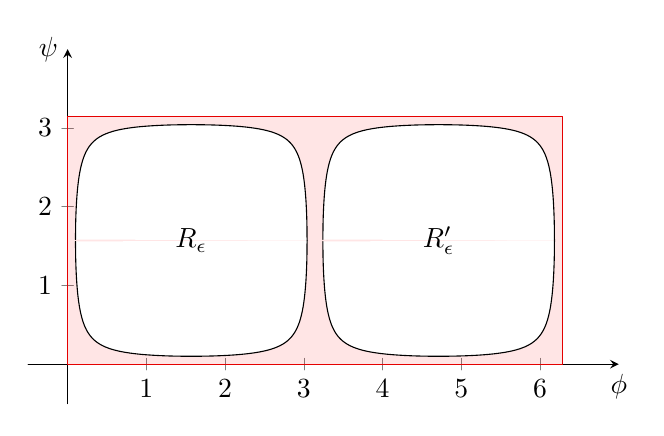
\begin{tikzpicture}[line cap=round,line join=round,>=triangle 45,x=1cm,y=1cm]
\begin{axis}[
	x=1cm,y=1cm,
	axis lines=middle,
	xmin=-0.5,
	xmax=7,
	ymin=-0.5,
	ymax=4,
	xtick={1,2,...,6},
	ytick={1,2,3},
	xlabel={$\phi$},
	x label style={anchor=north},
	ylabel={$\psi$},
	y label style={anchor=east}
]

\draw [color=red] (0,0) -- (2*pi,0) -- (2*pi,pi) -- (0,pi) -- cycle;
\draw [fill=red, opacity=0.1] (0,0) -- (2*pi,0) -- (2*pi,pi) -- (0,pi) -- cycle;

\addplot [smooth, fill=white, samples=100, domain=-0.9949874:0.9949874] ({acos(x/sqrt(0.1^2+x^2))*pi/180},{acos(sqrt(1-x^2-0.1^2))*pi/180});
\addplot [smooth, fill=white, samples=100, domain=-0.9949874:0.9949874] ({acos(x/sqrt(0.1^2+x^2))*pi/180},{acos(-sqrt(1-x^2-0.1^2))*pi/180});

\addplot [smooth, fill=white, samples=100, domain=-0.9949874:0.9949874] ({acos(x/sqrt(0.1^2+x^2))*pi/180+pi},{acos(sqrt(1-x^2-0.1^2))*pi/180});
\addplot [smooth, fill=white, samples=100, domain=-0.9949874:0.9949874] ({acos(x/sqrt(0.1^2+x^2))*pi/180+pi},{acos(-sqrt(1-x^2-0.1^2))*pi/180});

\draw (0.5*pi,0.5*pi) node {$R_\epsilon$};
\draw (1.5*pi,0.5*pi) node {$R'_\epsilon$};
]
\end{axis}
\end{tikzpicture}

\end{center}
\caption{Parametric plot of the vertical slices on a sphere. The curve enclosing $R_\epsilon$ parametrizes the circle with $y=\epsilon$ and the curve enclosing $R'_\epsilon$ parametrizes the circle with $y=-\epsilon$. The plot here shows $\epsilon=0.1$. The light red area is the to area we want to calculate.}
\label{fig:borelkol-coor}
\end{figure}

To calculate the probability mass on $R_\epsilon$, we need Green's theorem. Define 
\begin{align*}
F(x)&=\begin{pmatrix}
\cos \psi(x)\\
0
\end{pmatrix},&r_{\pm}(x)&=\begin{pmatrix}\phi(x)\\\psi(x)\end{pmatrix}=\begin{pmatrix}\arccos\left(\frac{x}{\sqrt{x^2+\epsilon^2}}\right)\\
\arccos\left(\pm\sqrt{1-x^2-\epsilon^2}\right)
\end{pmatrix},
\end{align*}
then after accounting for orientation Green's theorem tells us
\begin{align*}
\P[R_\epsilon]&=\frac{1}{4\pi}\iint_{R_\epsilon}\sin\psi d\phi d\psi=\int_{r_-} F\cdot dr_- - \int_{r_+} F\cdot dr_+\\
&=\frac{1}{4\pi}\left(\int_{-\sqrt{1-\epsilon^2}}^{\sqrt{1-\epsilon^2}}\cos(\arccos(-\sqrt{1-x^2-\epsilon^2}))\cdot-\frac{\epsilon}{\epsilon^2+x^2}dx- \int F\cdot dr_+\right)\\
&=\frac{1}{4\pi}\left(\int_{-\sqrt{1-\epsilon^2}}^{\sqrt{1-\epsilon^2}}\frac{\epsilon\sqrt{1-x^2-\epsilon^2}}{\epsilon^2+x^2}dx- \int_{-\sqrt{1-\epsilon^2}}^{\sqrt{1-\epsilon^2}}-\frac{\epsilon\sqrt{1-x^2-\epsilon^2}}{\epsilon^2+x^2}dx\right)\\
&=\frac{2\epsilon}{4\pi}\int_{-\sqrt{1-\epsilon^2}}^{\sqrt{1-\epsilon^2}}\frac{\sqrt{1-x^2-\epsilon^2}}{\epsilon^2+x^2}dx.
\end{align*}
The latter integral can be calculated explicitly:
\begin{align*}
&\phantom{=}\int_{-\sqrt{1-\epsilon^2}}^{\sqrt{1-\epsilon^2}}\frac{\sqrt{1-x^2-\epsilon^2}}{\epsilon^2+x^2}dx\\
&=\left[\frac{1}{\epsilon}\arctan\left(\frac{x}{\epsilon\sqrt{1-x^2-\epsilon^2}}\right)-\arctan\left(\frac{x}{\sqrt{1-x^2-\epsilon^2}}\right)\right]_{-\sqrt{1-\epsilon^2}}^{\sqrt{1-\epsilon^2}}\\
&=\frac{1}{\epsilon}\cdot\frac{\pi}{2}-\frac{\pi}{2}-\left(\frac{1}{\epsilon}\cdot\frac{-\pi}{2}-\frac{-\pi}{2}\right)=\frac{\pi}{\epsilon}-\pi.
\end{align*}
We can now conclude that
\[\P[M'_\epsilon]=1-2\P[R_\epsilon]=1-2\cdot\frac{2\epsilon}{4\pi}\int_{-\sqrt{1-\epsilon^2}}^{\sqrt{1-\epsilon^2}}\frac{\sqrt{1-x^2-\epsilon^2}}{\epsilon^2+x^2}dx=\epsilon.\]
Note that this is equal to the probability mass on $C'_\epsilon$, the horizontal slice with height $\epsilon$ from the equator. Let $\epsilon'=\arcsin(\epsilon)$, then the horizontal slice equals $C'_\epsilon=[0,2\pi]\times\left[\frac{1}{2}\pi-\epsilon',\frac{1}{2}\pi+\epsilon'\right]$, after which
\begin{align*}
\P[C'_\epsilon]&=\frac{1}{4\pi}\int_0^{2\pi}b\int_{\frac{1}{2}\pi-\epsilon'}^{\frac{1}{2}\pi+\epsilon'}\sin\psi d\psi d\phi\\
&=\frac{1}{2}\cos\left(\frac{1}{2}\pi-\epsilon'\right)-\cos\left(\frac{1}{2}\pi+\epsilon'\right)=\sin\epsilon'\\
&=\epsilon=\P[M'_\epsilon].
\end{align*}
Since $M'_\epsilon$ is only a rotation on $C'_\epsilon$ and $\P$ is the uniform probability measure on the sphere, the equality of $\P[M'_\epsilon]$ and $\P[C'_\epsilon]$ is as expected.

\paragraph{A subset of the big slice}
We'll now consider subsets of the big slices $M'_\epsilon$. Let $a\in\left[0,\frac{1}{2}\pi\right]$ and $b\in\left[\frac{1}{2}\pi,\pi\right]$, then we'll consider the condition that $\psi\in[a,b]$. To make matters more simple we'll let $\phi\in\left[\frac{1}{2}\pi,\frac{3}{2}\pi\right]$. Figure~\ref{fig:borelkol-coor2} provides a visual representation of our calculations.

\begin{figure}
\begin{center}
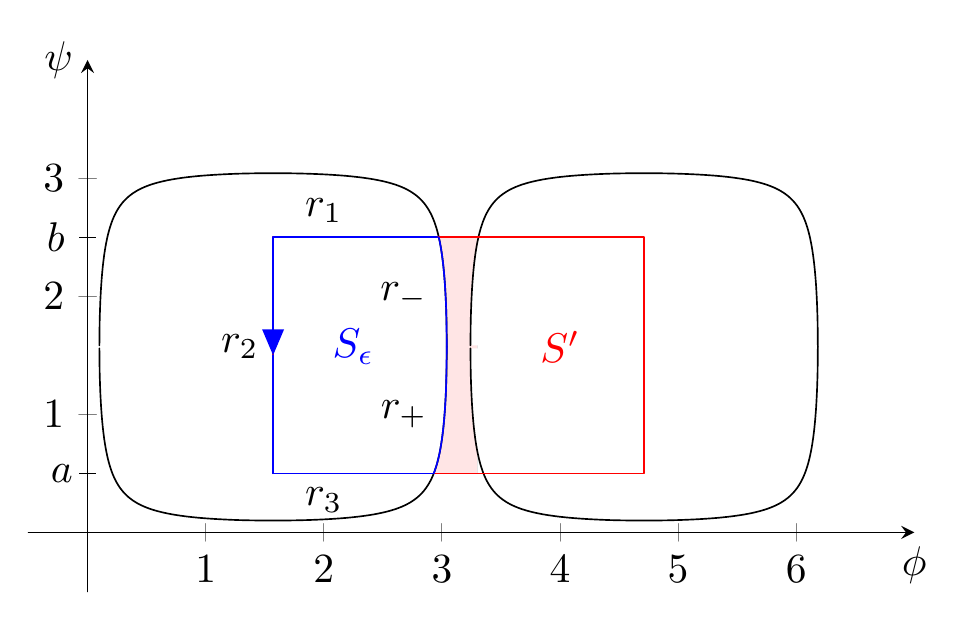
\begin{tikzpicture}[scale=1.5,line cap=round,line join=round,>=triangle 45,x=1cm,y=1cm]
\begin{axis}[
	x=1cm,y=1cm,
	axis lines=middle,
	xmin=-0.5,
	xmax=7,
	ymin=-0.5,
	ymax=4,
	xtick={1,2,...,6},
	ytick={1,2,3},
	xlabel={$\phi$},
	x label style={anchor=north},
	ylabel={$\psi$},
	y label style={anchor=east}
]

\draw [fill=red, opacity=0.1] (2.93146682,0.5) -- (3.3,0.5) -- (3.3,2.5) -- (2.93146682,2.5) -- cycle;

\addplot [smooth, fill=white, samples=100, domain=-0.9949874:0.9949874] ({acos(x/sqrt(0.1^2+x^2))*pi/180},{acos(sqrt(1-x^2-0.1^2))*pi/180});
\addplot [smooth, fill=white, samples=100, domain=-0.9949874:0.9949874] ({acos(x/sqrt(0.1^2+x^2))*pi/180},{acos(-sqrt(1-x^2-0.1^2))*pi/180});

\addplot [smooth, fill=white, samples=100, domain=-0.9949874:0.9949874] ({acos(x/sqrt(0.1^2+x^2))*pi/180+pi},{acos(sqrt(1-x^2-0.1^2))*pi/180});
\addplot [smooth, fill=white, samples=100, domain=-0.9949874:0.9949874] ({acos(x/sqrt(0.1^2+x^2))*pi/180+pi},{acos(-sqrt(1-x^2-0.1^2))*pi/180});

\draw [color=red] (0.5*pi,0.5) -- (1.5*pi,0.5) -- (1.5*pi,2.5) -- (0.5*pi,2.5) -- cycle;

\draw [color=blue] (0.5*pi,0.5) -- (2.93146682,0.5);
\draw [color=blue] (0.5*pi,2.5) -- (2.96,2.5);
\draw [color=blue] (0.5*pi,0.5) -- (0.5*pi,1.5);
\draw [color=blue, ->] (0.5*pi,2.5) -- (0.5*pi,1.5);

\addplot [smooth, color=blue, samples=10, domain=-0.9949874:-0.46888] ({acos(x/sqrt(0.1^2+x^2))*pi/180},{acos(sqrt(1-x^2-0.1^2))*pi/180});
\addplot [smooth, color=blue, samples=10, domain=-0.9949874:-0.59] ({acos(x/sqrt(0.1^2+x^2))*pi/180},{acos(-sqrt(1-x^2-0.1^2))*pi/180});

\draw (2,2.5) [above] node {$r_1$};
\draw (0.5*pi,0.5*pi) [left] node {$r_2$};
\draw (2,0.5) [below] node {$r_3$};
\draw (3,2) [left] node {$r_-$};
\draw (3,1) [left] node {$r_+$};

\draw [color=blue] (2.25,0.5*pi) node {$S_\epsilon$};
\draw [color=red] (4,0.5*pi) node {$S'$};

\draw [line width=0mm] (-2pt,0.5) -- (2pt,0.5);
\draw (0,0.5) node [left] {$a$};
\draw [line width=0mm] (-2pt,2.5) -- (2pt,2.5);
\draw (-2pt,2.5) node [left] {$b$};
]
\end{axis}
\end{tikzpicture}

\end{center}
\caption{Parametric plot of the vertical slices on a sphere. This plot is equal to figure~\ref{fig:borelkol-coor}. The light red area is the area we want to calculate. This will be done by calculating area $S_\epsilon$, enclosed by the blue curve. The area $S'$ is enclosed by the red rectangle, which partly coincides with the blue curve.}
\label{fig:borelkol-coor2}
\end{figure}

Let $S'=\left[\frac{1}{2}\pi,\frac{3}{2}\pi\right]\times[a,b]$ and let 
\[E'_\epsilon=S'\setminus\left(R_\epsilon\cup R'_\epsilon\right)\subseteq M'_\epsilon,\]
then $E'_\epsilon$ corresponds to the light red area in figure~\ref{fig:borelkol-coor2}. By symmetry of the probability mass in $\phi=\pi$ we have \[\P[E'_\epsilon]=\P[S']-2\P[S_\epsilon].\]

We'll start with the calculation of $\P[S']$. This calculation is quite simple:
\[\P[S']=\frac{1}{4\pi}\int_{\frac{1}{2}\pi}^{\frac{3}{2}\pi}\int_a^b\sin\psi d\psi \phi=\frac{1}{4}(\cos a-\cos b).\]

For the area $\P[S_\epsilon]$ Green's theorem is again needed. We'll use the same vector field $F=(\cos\psi,0)^\top$. Parametrize all five curves as the following:
\begin{align*}
r_-(x)&=\begin{pmatrix}
\arccos\left(\frac{x}{\sqrt{x^2+\epsilon^2}}\right)\\
\arccos\left(-\sqrt{1-x^2-\epsilon^2}\right)
\end{pmatrix},&x&\in\left[-\sqrt{1-\epsilon^2},-\sqrt{\sin(b)^2-\epsilon^2}\right],\\
r_+(x)&=\begin{pmatrix}
\arccos\left(\frac{x}{\sqrt{x^2+\epsilon^2}}\right)\\
\arccos\left(\sqrt{1-x^2-\epsilon^2}\right)
\end{pmatrix},&x&\in\left[-\sqrt{1-\epsilon^2},-\sqrt{\sin(a)^2-\epsilon^2}\right],\\
r_1(\phi)&=\begin{pmatrix}\phi\\b\end{pmatrix},&\phi&\in\left[\frac{1}{2}\pi,\arccos\left(-\sqrt{1-\frac{\epsilon^2}{\sin(b)^2}}\right)\right],\\
r_2(\psi)&=\begin{pmatrix}\frac{1}{2}\pi\\\psi\end{pmatrix},&\psi&\in[a,b],\\
r_3(\phi)&=\begin{pmatrix}\phi\\a\end{pmatrix},&\phi&\in\left[\frac{1}{2}\pi,\arccos\left(-\sqrt{1-\frac{\epsilon^2}{\sin(a)^2}}\right)\right].
\end{align*}
Checking the correctness of these parameterizations is left as an exercise for the reader.

In this case Green's theorem, keeping counterclockwise orientation into account, gives
\begin{align*}
4\pi\P[S_\epsilon]&=\iint_{S_\epsilon}\sin\psi d\phi d\psi\\
&=\int_{r_-}F\cdot dr_- -\int_{r_1} F\cdot dr_1-\int_{r_2}F\cdot dr_2+\int_{r_3}F\cdot r_3-\int_{r_+}F\cdot dr_+.
\end{align*}
We'll now calculate each integral, starting the ones over $r_1$, $r_2$ and $r_3$.

The easiest integral is over $r_2$. We have $dr_2(\psi)=(0,1)^\top$, thus 
\[\int_{r_2}F\cdot dr_{2}=\int_a^b\cos(\psi)\cdot0d\psi=0.\]
Consider now the integrals over $r_1$ and $r_3$. They provide
\begin{align*}
\int_{r_1}F\cdot dr_1&=\int_{\frac{1}{2}\pi}^{\arccos\left(-\sqrt{1-\frac{\epsilon^2}{\sin(b)^2}}\right)}\cos (b) d\psi\\
&=\cos b\left(\arccos\left(-\sqrt{1-\frac{\epsilon^2}{\sin(b)^2}}\right)-\frac{1}{2}\pi\right),\\
\int_{r_3}F\cdot dr_3&=\int_{\frac{1}{2}\pi}^{\arccos\left(-\sqrt{1-\frac{\epsilon^2}{\sin(a)^2}}\right)}\cos (a) d\psi\\
&=\cos a\left(\arccos\left(-\sqrt{1-\frac{\epsilon^2}{\sin(a)^2}}\right)-\frac{1}{2}\pi\right).
\end{align*}
Taking $\epsilon\to0$ gives 
\begin{align*}
\lim_{\epsilon\to0}\int_{r_1}F\cdot dr_1&=\cos b\left(\arccos(-1)-\frac{1}{2}\pi\right)=\frac{1}{2}\pi\cos b,\\
\lim_{\epsilon\to0}\int_{r_3}F\cdot dr_3&=\cos a\left(\arccos(-1)-\frac{1}{2}\pi\right)=\frac{1}{2}\pi\cos a.
\end{align*}

This leaves us the integrals over $r_-$ and $r_+$. Both are already calculated, but with different bounds. Furthermore, note that
\begin{align*}
F\cdot dr_-&=\frac{\epsilon\sqrt{1-x^2-\epsilon^2}}{\epsilon^2+x^2}dx=-\frac{-\epsilon\sqrt{1-x^2-\epsilon^2}}{\epsilon^2+x^2}dx=-F\cdot dr_+,
\end{align*}
thus the integrands of $\int_{r_-}F\cdot dr_-$ and $\int_{r_+}F\cdot dr_+$ are each opposites. Therefore we only need to calculate only one integral explicitly to solve both. We'll keep our focus on $r_-$ for now. This integral equals
\begin{align*}
&\phantom{=}\int_{r_-}F\cdot dr_-=\int_{-\sqrt{1-\epsilon^2}}^{-\sqrt{\sin(b)^2-\epsilon^2}}\frac{\epsilon\sqrt{1-x^2-\epsilon^2}}{\epsilon^2+x^2}dx\\
&=\left[\arctan\left(\frac{x}{\epsilon\sqrt{1-x^2-\epsilon^2}}\right)-\epsilon\arctan\left(\frac{x}{\sqrt{1-x^2-\epsilon^2}}\right)\right]_{-\sqrt{1-\epsilon^2}}^{-\sqrt{\sin(b)^2-\epsilon^2}}\\
&=\arctan\left(-\frac{1}{\epsilon}\sqrt{\frac{\sin(b)^2-\epsilon^2}{\cos(b)^2}}\right)-\epsilon\arctan\left(-\sqrt{\frac{\sin(b)^2-\epsilon^2}{\cos(b)^2}}\right)+\frac{\pi}{2}\left(1-\epsilon\right).
\end{align*}
When letting $\epsilon\to0$ we only need to look at $\lim_{\epsilon\to0}\arctan\left(-\frac{1}{\epsilon}\sqrt{\frac{\sin(b)^2-\epsilon^2}{\cos(b)^2}}\right)$, as the other terms either stay constant or vanish. In this case
\begin{align*}\lim_{\epsilon\downarrow0}\arctan\left(-\frac{1}{\epsilon}\sqrt{\frac{\sin(b)^2-\epsilon^2}{\cos(b)^2}}\right)&=\lim_{\epsilon\downarrow0}\arctan\left(-\sqrt{\frac{\tan^2(b)}{\epsilon^2}-\frac{1}{\cos(b)^2}}\right)\\
&=\lim_{x\to\infty}\arctan(-x)=-\frac{\pi}{2}.
\end{align*}
Therefore
\[\lim_{\epsilon\downarrow0}\int_{r_-}F\cdot dr_-=\frac{-\pi}{2}-0+\frac{\pi}{2}-0=0.\]

The negative integral $-\int_{r_+}F\cdot dr_+$ is equal to $\int_{r_-}F\cdot dr_-$, except all $b$'s are replaced by $a$. This integral vanishes as well when taking $\epsilon\to0$.

Now we have calculated all parts of $\P[S_\epsilon]$, we can try to find an expression for $\lim_{\epsilon\downarrow0}\P[S_\epsilon]$:
\begin{align*}
&\phantom{=}\lim_{\epsilon\downarrow0}4\pi\P[S_\epsilon]\\
&=\lim_{\epsilon\downarrow0}\left(\int_{r_-}F\cdot dr_- -\int_{r_1} F\cdot dr_1-\int_{r_2}F\cdot dr_2+\int_{r_3}F\cdot r_3-\int_{r_+}F\cdot dr_+\right)\\
&=0-\frac{1}{2}\pi\cos b-0+\frac{1}{2}\pi\cos a-0\\
&=\frac{1}{2}\pi\left(\cos a-\cos b\right).
\end{align*}
This concludes to
\[\lim_{\epsilon\downarrow0}\P[E'_\epsilon]=\P[S']-2\lim_{\epsilon\downarrow0}\P[S_\epsilon]=\frac{1}{4}(\cos a-\cos b)-\frac{1}{4}(\cos a-\cos b)=0,\]
which is just as expected. Furthermore, using the same calculations as for the big slice, $\P[E'_\epsilon]$ is expected to equal
\[\P[E'_\epsilon]=\frac{b-a}{2\pi}\epsilon.\]
It is either not possible or extremely complicated to prove this from the expression we've found for $\P[E'_\epsilon]$. However, firstly $\P[E'_\epsilon]=\frac{b-a}{2\pi}\epsilon$ should hold as it is a mere rotation of a piece of a slice on the equator and after calculating the found $\P[E'_\epsilon]$ and $\frac{b-a}{2\pi}{\epsilon}$ for various $a\in[0,\frac{1}{2}\pi]$, $b\in\left[\frac{1}{2}\pi,\pi\right]$ and $\epsilon\in(0,0.1)$ we find that both are equal in all tested cases. Therefore it is safe to assume that $\P[E'_\epsilon]=\frac{b-a}{2\pi}\epsilon$ holds without a rigorous proof.

\paragraph{Combining both results}
We can now combine both results to find out the limit of $\P[E'_\epsilon|M'_\epsilon]$. Since $E'_\epsilon\subset M'_\epsilon$, it suffices to consider the limit of $\frac{\P[E'_\epsilon]}{\P[M'_\epsilon]}$ with $\epsilon\downarrow 0$. Recall that $\P[M'_\epsilon]=\epsilon$ and $\P[E'_\epsilon]=\frac{b-a}{2\pi}{\epsilon}$, therefore
\[\P[E'_0|M'_0]=\lim_{\epsilon\downarrow0}\frac{\P[E'_\epsilon]}{\P[M'_\epsilon]}=\lim_{\epsilon\downarrow0}\frac{\frac{b-a}{2\pi}\epsilon}{\epsilon}=\frac{b-a}{2\pi}.\]

This leaves the conclusion that conjecture~\ref{con:conditional} is false, since we have two conditional probabilities on $\{\pi\}\times[a,b]$ given $\{0,\pi\}\times[0,\pi]$. When considering the limit of meridians the conditional probability is $\frac{1}{4}(\cos a-\cos b)$, while considering the limit of vertical slices the conditional probability becomes $\frac{b-a}{2\pi}$.

This leaves only one conclusion: the conditional probability distribution on a zero set is not uniquely determinable by converging sequences in sub-$\sigma$-algebras.

This leaves the Borel-Kolmogorov paradox wide open, with the only satisfiable conclusion for the conditional probability that it depends on the chosen parametrization and can be anything from $0$ to $1$. When considering the conditional probability of a section $C$ on a great circle, we can parametrize meridians with a pole on $C$, creating a low density, or we can parametrize longitudes to attain a uniform distribution. The only assurance is that after having chosen an arbitrary parametrization to compute the conditional density on $C$, this parametrization must be able to extend to the sphere and to retrieve the uniform distribution there.
\section{Two envelope problem}
Another paradox to consider is the two envelope problem. This problem is first stated by \cite{Kraitchik53} as the necktie problem. There each person claims to have the finer necktie. A judge must make a decision, where the winner must give his necktie to the loser. The argument of the each contestant is `I know what my tie is worth. I may lose it, but I may also win a better one, so the game is to my advantage.' However, a game that is favorable for both players cannot exist. Furthermore, the game is symmetrical in terms of the contestants, thus \cite{Kraitchik53} states that the chance of winning is actually $\frac{1}{2}$.

However, \cite{Kraitchik53} only provides a discussion and no rigorous proofs. In 1989 \cite{Nalebuff89} states the two envelope problem and provides a wide discussion. We will consider one of the variants, in my opinion the simplest, of the paradox and remove all paradoxical statements. The reasoning will stay valid for various extensions to the problem.

The two envelope problem stated by \cite{Nalebuff89} is as follows. There are two envelopes, $A$ and $B$. Envelope $A$ contains a fixed amount of money and envelope $B$ contains either $\frac{1}{2}A$ or $2A$ amount of money. The player can choose between envelope $A$ or $B$ and let us say without loss of generality he chooses envelope $A$. After choosing, the player is given the choice whether he must switch. He reasons that envelope $B$ contains $\frac{1}{2}A$ with probability $\frac{1}{2}$ and $2A$ with probability $\frac{1}{2}$, thus \[\E[B]=\frac{1}{2}\cdot\frac{1}{2}A+\frac{1}{2}\cdot2A=\frac{5}{4}A\] is the expected value of money in envelope $B$. Thus the player always wants to switch. However, by symmetry, if the player has chosen envelope $B$, then to his knowledge $A$ either contains $\frac{1}{2}B$ or $2B$, thus he also wants to switch. If the player possesses no memory, then he will switch infinitely many times, believing to gain infinite money.

\subsection{Fixing expectation values}
The two envelope problem asks where the flaw is in the reasoning above. The biggest flaw is in the calculation of $\E[B]$, this calculation is performed using incorrect probability measures. An in-depth discussion can be found in \cite{Brien14}, we'll only provide the problem's core resolution.

The envelopes can only obtain two values: $x$ and $2x$. The probability of $A$ having $x$ is $\frac{1}{2}$, thus the probability space is \[\left(\X=\{(x,2x),(2x,x)\},\F=2^\X,\P\right)\] with $\P$ the probability measure such that $\P[\{(x,2x)\}]=\P[\{(2x,x)\}]=\frac{1}{2}$. The calculation of $\E[B]$ in the statement of the two envelope problem is the following:
\[\E[B]=\frac{A}{2}\P\left[B=\frac{A}{2}\right]+2A\P[B=2A].\]
This calculation cannot be seen as valid, as $\left(A,\frac{A}{2}\right)$ is not present in our probability space. The following calculation inspired by \cite{Schwitzgebel08} and \cite{Brien14} is correct:
\begin{align*}
\E[B]&=\E[\E[B|A]]=\E[B|A=x]\P[A=x]+\E[B|A=2x]\P[A=2x]\\
&=\frac{1}{2}\left(2x\P[B=2x|A=2x]\right)+\frac{1}{2}\left(x\P[B=2x|A=x]\right)\\
&=\frac{1}{2}\cdot2x+\frac{1}{2}x=\frac{3}{2}x.
\end{align*}
We can calculate in the same way that $\E[A]=\frac{3}{2}x$, thus the expected amount of money in either envelope is equal. Switching therefore does not increase ones chances of getting more money.

\subsection{Prior on envelope values}

This discussion however does not completely resolve the two envelope paradox. Two immediate flaws can be found in the discussion given:
\begin{enumerate}
\item How is the value $x$ picked? If the value $x$ is drawn from a probability distribution on an unbounded set $U$, then it is not possible for all $x\in U$ that $\P[B=2x|A=x]=\P\left[B=\frac{1}{2}x\middle|A=x\right]=\frac{1}{2}$, as that would imply that $\P$ is the uniform distribution on $U$. It is clear that uniform distributions on unbounded sets do not exist. If the value $x$ is in some other way picked from a possibly singular probability distribution, then it could give some information whether the player must switch, as in those cases the inequality $\P[B=2x|A=x]\neq\P\left[B=\frac{1}{2}x\middle|A=x\right]$ holds as well more often that not.
\item Expanding on the previous point, if $x$ is drawn from a probability distribution with $\E[B]=\E[A]=\infty$, then $\E[B]=\E[\E[B|A]]$ is in some cases not valid any more \cite{Tzur18}.
\end{enumerate}

To fully resolve the two envelope paradox, we must expand our probability space. To be precise, we must enforce a prior $f$ on the lowest value $x$ in either envelope. For the full analysis, we will rephrase the two envelope problem.

The game master draws a value $X$ from a prior distribution $f$. He then draws a random variable $U$ from $\{0,1\}$ and puts $(1+U)X$ in envelope $A$ and $(2-U)X$ in envelope $B$. Envelope $A$ is given to the player. The player inspects his envelope and observes a value $y$. The game master then asks the player whether he wants to switch to envelope $B$.

Note that envelope $A$ is given to the player, not that the player is able to choose between envelopes $A$ and $B$. Both games are in fact the same by symmetry, as one of the two envelopes is given to the player and before opening an envelope, the player cannot favour one envelope above the other.

This game is studied extensively and has many variants, such as whether $\E[X]=\infty$ or not, whether distribution $f$ is heavy-tailed, etcetera. We will take a look at various variations, starting from the player having full information on $f$ and then removing information for the player, ending up in a strategy where the player must guess the expectation and variance of $f$ and then is able to gain long run profit from this game.

\subsubsection{The prior's influence}
Define the gain $G=B-A$. In this case it is easy to see that
\[\E[G]=\E[B]-\E[A]=(2-\E[U])\E[X]-(1+\E[U])\E[X]=0.\]
We are interested in the gain given the information in envelope $A$. To be precise, we want to model $G|A=a$. We'll take a look at a few examples on how the prior on $X$ can influence $G|A=a$.

\begin{example}[\cite{Navara2017}]
The following example is taken from \cite{Navara2017}. Assume that $f$ is a discrete prior, then we can follow the analysis of \cite{Navara2017}. There they assume $\E[U]=\P[U=1]=\frac{1}{2}$.

First we'll want to know how much we expect to gain, given value $a$ is in envelope $A$. The expectation value of $G|A=a$ is 
\[\E[G|A=a]=\frac{af(a)-\frac{a}{2}f\left(\frac{a}{2}\right)}{f(a)+f\left(\frac{a}{2}\right)}.\]
When a prior $f(2^t)=\frac{q^t}{1-q}$, three different cases can be distinguished:
\begin{enumerate}
	\item[$q<\frac{1}{2}$:] Suppose $q<\frac{1}{2}$, then $\E[X]$ exists and is equal to $\E[X]=(1-q)^{-1}(1-2q)^{-1}$. In this case we have
	\[\E\left[G\middle|A=2^t\right]=\begin{cases}2^{t-1}\frac{2q-1}{q+1},&t\in\N_{\geq 1}\\1,&t=0.\end{cases}\]
	Therefore with this prior switching is only recommended when one observes a value of $1$ in his envelope.
	\item[$q=\frac{1}{2}$:] Suppose $q=\frac{1}{2}$, then $\E[X]$ does not exist any more. The expected gain now simplifies to $\E\left[G\middle|A=2^t\right]=\1_{\{0\}}(t)$, thus there is only gain on switching when $A=1$.
	\item[$q>\frac{1}{2}$:] Suppose $q>\frac{1}{2}$, then $\E[X]$ does not exist as well. The conditional gain $G|A=2^t$ is still valid and equals
	\[\E\left[G\middle|A=2^t\right]=\begin{cases}2^{t-1}\frac{2q-1}{q+1},&t\in\N_{\geq 1}\\1,&t=0.\end{cases},\]
	which is strictly positive for all $s\in\N$. Thus the player is motivated to always switch, resulting in again a paradox.
\end{enumerate}

Therefore the $q$ controlling the prior $f$ can lead to various results, from non-paradoxical advise to only switch when obtaining the smallest value $1$, knowing the other envelope must contain $2$, to the original paradox of always having to switch, no matter the contents of $A$. The difference with the original paradox is that the latter paradox is supported by a prior on $X$, not by wrongly interpreting the statement of the problem.
\end{example}

\begin{example}[\cite{Broome95}]
Consider first the discrete case. Let $f(2^n)=\frac{2^n}{3^{n+1}}$ be a prior for all $n\in\N_{\geq 0}$. We now want to know the expected value of $y$ in envelope $B$. The trivial case is $\E[B|A=1]=2$, as the only possible value in envelope $B$ is $2$ when observing $1$.\\
Suppose we observe a value $a\neq1$. Then we have $x=a$ or $x=\frac{1}{2}a$. The probability of $B$ having $2a$ becomes
\begin{align*}
\P[B=2a|A=a]&=\P\left[X=a\middle|X=a\lor X=\frac{a}{2}\right]\\
&=\frac{\frac{2^n}{3^{n+1}}}{\frac{2^n}{3^{n+1}}+\frac{2^{n-1}}{3^{n}}}=\frac{2}{5}.
\end{align*}
Then we have $\P\left[B=\frac{a}{2}\middle|A=a\right]=1-\P[B=2a|A=a]=\frac{3}{5}$, giving an expected value of envelope $B$ of
\[\E[B|A=a]=\frac{2}{5}\cdot2a+\frac{3}{5}\cdot\frac{a}{2}=\frac{11}{10}a.\]
The paradoxical conclusion is that the player must always switch, no matter the contents of his envelope. The reason why $\E[B|A=a]>0$ for all $a=2^n$ is possible, is that $\E[X]=\sum_{n=1}^\infty\left(\frac{4}{3}\right)^n=\infty$ holds.

For now we've only seen discrete distributions, but paradoxical conclusions can result from continuous distributions as well. Let $f$ be the density function of the prior on $X$, then
\[\E[B|A=a]=a\frac{8f(a)+f\left(\frac{a}{2}\right)}{4f(x)+2f\left(\frac{a}{2}\right)}.\]
Take density function $f(x)=(x+1)^{-2}$ with $x\in[0,\infty)$, then 
\[\E[B|A=a]=a\frac{2(a+2)^2+(a+1)^2}{(a+2)^2+2(a+1)^2}>0\]
holds for all $a\in[0,\infty)$. Here the situation that switching is advised arises as well. Note that the expectation value of the prior is $\E[X]=\int_0^\infty \frac{x}{(x+1)^2}dx=\infty$, explaining why $\E[B|A=a]>0$ for all $a\in(0,\infty)$ is again possible.
\end{example}

When considering $\E[G|A=a]$, one can quantify when a distribution yields paradoxical results. For discrete priors, $\E[G|A=a]$ equals \cite{Navara2017,Tzur18} 
\[\E[G|A=a]=\frac{af(a)-\frac{a}{2}f\left(X=\frac{a}{2}\right)}{f(a)+f\left(\frac{a}{2}\right)},\]
where it gives rise to the following definition.
\begin{definition}[Paradoxical distribution]
A discrete prior $f$ on $X$ is called \emph{paradoxical} if $f(x)>\frac{1}{2}f\left(\frac{x}{2}\right)$ holds for all $x\in\N$.
\end{definition}
\begin{lemma}
Let $f$ be a discrete paradoxical distribution on $X$, then $\E[X]=\infty$.
\end{lemma}
\begin{proof}
This proof is taken from \cite{Tzur18}. Let $x$ be a possible realization of $X$, then $2^k x$ with $k\in\N$ are possible realizations of $X$ as well by the setting of the two envelope problem. Then $2^{k+1}xf(2^{k+1} x)>2^x xf(2^kx)$ holds for all $x\in\N$, implying unbounded $\E[X]=\sum_{k=0}^\infty k f(k)>\sum_{k=0}^\infty 2^k xf(2^k x).$
\end{proof}

We will from now on cover both paradoxical as non-paradoxical distributions. It is now clear that, when having full information, paradoxical distributions still yield unexpected results. However, this is contributed to the expectation value of the prior being undefined, not to a wrong interpretation of the problem. When having full information non-paradoxical priors yield well-defined switching strategies.

\subsubsection{Optimal solution}
Suppose a non-paradoxical prior on $X$ is known, does an optimal switching strategy exist? This question is asked and answered by \cite{Christensen92} and further discussed by \cite{Christensen93a,Christensen93b,Christensen94,Christensen96}. Originally, \cite{Christensen92} proposed a solution for all general priors, however \cite{Christensen96} pointed out this is incorrect for continuous distributions. Here we'll combine the discussion and immediately provide a resolution.

\paragraph{Discrete priors}
Let $f$ be a discrete prior on $X$. Then \cite{Christensen92} calculates that
\begin{align*}
\P\left[X=a\middle|A=a\right]&=\frac{\P[A=a|X=a]f(a)}{\P[A=a|X=a]f(a)+\P\left[A=a\middle|X=\frac{a}{2}\right]f\left(\frac{a}{2}\right)}\\
&=\frac{f(a)}{f(a)+f\left(\frac{a}{2}\right)},\\
\P\left[X=\frac{a}{2}\middle|A=a\right]&=\frac{\P\left[A=a\middle|X=\frac{a}{2}\right]f\left(\frac{a}{2}\right)}{\P[A=a|X=a]f(a)+\P[A=a|X=2a]f(2a)}\\
&=\frac{f\left(\frac{a}{2}\right)}{f(a)+f\left(\frac{a}{2}\right)},\\
\end{align*}
To compute $\E[B|A=a]$, note that there are two possibilities: either $B=2a$, which happens when $X=a$ upon seeing $A=a$ or $B=\frac{a}{2}$ when $X=\frac{a}{2}$ upon seeing $A=a$. Therefore
\begin{align*}
\E[B|A=a]&=\frac{a}{2}\P\left[X=\frac{a}{2}\middle|A=a\right]+2a\P\left[X=a\middle|A=a\right]\\
&=\frac{af\left(\frac{a}{2}\right)+4af(a)}{2f(a)+2f\left(\frac{a}{2}\right)}.
\end{align*}
Obviously when $\E[B|A=a]>a$ holds, switching is advised, which happens when $f\left(\frac{a}{2}\right)<2f(a)$.

First we'll review the paradox with the aforementioned background. The original paradox arises from the fact that \[\P[B=2a|A=a]=\P\left[B=\frac{a}{2}\middle|A=a\right]=\frac{1}{2}\] is assumed for all possible values $a$. This however cannot be possible, as in this case the prior $f$ must be a flat on all integers \cite{Christensen92,Christensen93b}.

The next question to ask is whether there is a prior $f$ for which the requirement $\E[B|A=a]\leq a$ holds for all $a$. The answer is no, as \cite{Brams95} points out in a quite simple proof. In order for $\E[B|A=a]\leq a$ we must have $f\left(\frac{a}{2}\right)\geq2f(a)$ for all $a$. Let $a$ be such that $f(a)>0$, then $f\left(a\right)\geq 2^{n}f(2^na)$ holds for all $n\in\Z$, leading to $f(a)\to0$ as $n\to-\infty$.

The last question we'll ask here is if there is a prior such that $\E[B|A=a]>a$ holds for all $a$. Then $f\left(\frac{a}{2}\right)>f(a)$ must hold for all $a$, which is achieved for all paradoxical distributions. Various examples can be found in \cite{Christensen93a,Linzer94,Broome95}, with $f(2^n)=\frac{2^n}{3^{n+1}}$ as the easiest one. In this case a new paradox arises, where switching is always advised. Note that Christensen and Utts do not agree with this being a paradox as stated in \cite{Christensen93a}, as $\E[B|A=a]$ is still finite and can be compared with $a$.
\paragraph{Continuous case}
Let $f$ be a continuous prior on $X$. First \cite{Christensen92} states that \[\E[B|A=a]=\frac{af\left(\frac{a}{2}\right)+4af(a)}{2f(a)+2f\left(\frac{a}{2}\right)}\] holds for continuous priors as well, however \cite{Christensen96} points out this is a mistake.

Take a look at the following analysis from \cite{Brams95}. Let $Y=\frac{X}{2}$ and let $g$ be a prior on $Y$. Then $\P[X\leq x]=\P\left[Y\leq \frac{x}{2}\right]$, thus $F(x)=G\left(\frac{x}{2}\right)$. Differentiating for the density functions yields $f(x)=\frac{1}{2}g\left(\frac{x}{2}\right)$. Now, analogous to the discrete case, we have
\begin{align*}
\P[X=a|A=a]&=\frac{f(x)}{f(x)+g(x)}=\frac{f(x)}{f(x)+\frac{1}{2}f\left(\frac{x}{2}\right)},\\
\P\left[X=\frac{a}{2}\middle|A=a\right]&=\frac{g(x)}{f(x)+g(x)}=\frac{\frac{1}{2}f\left(\frac{x}{2}\right)}{f(x)+\frac{1}{2}f\left(\frac{x}{2}\right)}.
\end{align*}
The expectation of $B|A=a$ now becomes
\begin{align*}
\E[B|A=a]&=\frac{a}{2}\P\left[X=\frac{a}{2}\middle|A=a\right]+2a\P\left[X=a\middle|A=a\right]\\
&=\frac{af\left(\frac{a}{2}\right)+8af(a)}{4f(a)+2f\left(\frac{a}{2}\right)}.
\end{align*}
This expectation value is different from \cite{Christensen96}, they made a mistake mixing up the probabilities while calculating the expectation value. Their conclusion that now $4f(a)>f\left(\frac{a}{2}\right)$ must hold in order to get $\E[B|A=a]$ is still correct.

As in the discrete case all continuous priors must have an $a$ such that $\E[B|A=a]>a$ holds \cite{Brams95}. Examples for which $\E[B|A=a]>a$ holds for all $a$ can be found in \cite{Christensen96,Broome95,Brams95}, with $f(a)=(a+1)^{-2}$ for $a\in(0,\infty)$ being one of the easiest examples \cite{Broome95}.

\subsubsection{Cover's switching strategy}
When playing the two envelope game, the player usually does not know the prior on the lowest value $X$. Is there a strategy such that upon seeing one envelope's value the player can choose to switch or not and on average receive more than $\frac{3}{2}x$, independent of the prior? The answer is yes, in fact infinitely many strategies exist. This question is briefly touched upon by \cite{Christensen92,Christensen94} and extended by \cite{McDonnell09,Abbott10,McDonnell11}. 

Assume that the prior $f$ on $X$ is continuous with finite mean. Recall that envelope $A$ receives $(U+1)X$ with $U\sim\mathrm{Ber}(1-p)$ Bernoulli distributed. After observing value $a$, the player randomly switches with probability $P(a)$. The key point is that strategies whether to switch or not can perfectly be modelled by probability distributions. Let $R$ be the value returned to the player at the end of the game, then
\begin{align*}
\P[R=x|X=x]&=\P[A=x|X=x](1-P(x))+\P[A=2x|X=x]P(2x)\\
&=p(1-P(x))+(1-p)P(2x),\\
\P[R=2x|X=x]&=\P[A=2x|X=x](1-P(2x))+\P[A=x|X=x]P(x)\\
&=(1-p)(1-P(2x))+pP(x).
\end{align*}
Therefore the conditional expectation of the return given $X=x$ is 
\begin{align*}
\E[R|X=x]&=x\P[R=x|X=x]+2x\P[R=2x|X=x]\\
&=x(2-p)+pxP(x)-x(1-p)P(2x)).
\end{align*}
Thus following \cite{McDonnell09} we get
\begin{align*}
\E[R]=\E[\E[R|X]]&=\int_0^\infty f(x)\E[R|X=x]dx\\
&=(2-p)\E[X]+\int_0^\infty xf(x)(pP(x)-(1-p)P(2x))dx.
\end{align*}
When the player never switches, his expected return is $(2-p)\E[X]$. Thus define $G=\int_0^\infty xf(x)(pP(x)-(1-p)P(2x))dx$ as the players gain of his switching strategy. One can immediately see that $pP(x)\geq(1-p)P(2x)$ for all $x$ is a sufficient condition for a non-negative gain. The gain can be rewritten as
\begin{align}
G&=\int_0^\infty xf(x)(pP(x)-(1-p)P(2x))dx\\
&=\int_0^\infty xP(x)\left(pf(x)-\frac{1-p}{4}f\left(\frac{x}{2}\right)\right)dx,\label{eq:gainprop}
\end{align}
where both representations will become useful in different manners.
\begin{theorem}[McDonnell, Abbott \cite{McDonnell09}]\label{thm:switchopt}
The optimal switching strategy $P^*(x)$ is 
\[P^*(x)=\1_{[0,\infty)}\left(pf(x)-\frac{1-p}{4}f\left(\frac{y}{2}\right)\right).\]
\end{theorem}


From now on we'll put $p=\frac{1}{2}$ as in our model an envelope is  distributed to the player uniformly. In this case $P(x)\geq P(2x)$ for all $x\in[0,\infty)$ is needed for non-negative gain. We'll now look at two example strategies, namely Cover switching and threshold switching. More examples, comparison between the examples and simulations of the examples can be found in \cite{McDonnell09,McDonnell11}.

\begin{example}[Cover switching]
This example is taken from \cite{McDonnell09,Abbott10}. Let $a\in(0,\infty]$ be arbitrary and put $P(x)=e^{-ax}$. This $P$ is called \emph{Cover switching}. The inequality $P(x)\geq P(2x)$ is automatically satisfied as the requirement $e^{-ax}>e^{-2ax}$ holds for all positive $x$.

Suppose that $X\sim\mathrm{Exp}(c)$ is exponentially distributed. Then switching using Cover's strategy is maximized for $a=\left(\frac{1}{3}\sqrt[3]{2}+\frac{1}{6}\sqrt[3]{4}-\frac{1}{3}\right)c$, with a return of $\E[R_C]=\frac{3\sqrt[3]{2}+3-3\sqrt[3]{4}}{c\sqrt[3]{2}}\approx\frac{1.6013}{c}$. The return of this prior for never or always switching strategy is $\E[R]=\frac{3}{2}\E[X]=\frac{3}{2c}$, thus Cover switching does improve on never or always switching.
\end{example}

\begin{example}[Threshold switching]
This example is taken from \cite{McDonnell09}. Let $b\in(0,\infty)$ be arbitrary and define $P(y)=\1_{[0,b]}(y)$. This strategy is called \emph{Threshold switching}. The player tries to switch all the low values he gets, but always holds on high values. Of course, if the prior on $X$ is unknown, no advice on which $b$ to choose can be given. However, as $P(x)\geq P(2x)$ always holds, this strategy has non-negative gain for all possible values $b$.

Let $X\sim\text{Exp}(c)$ be exponentially distributed. Looking at \eqref{eq:gainprop}, we want that $P(x)=1$ when $f(x)\geq\frac{1}{4}f\left(\frac{x}{2}\right)$ holds, thus when $ce^{-cx}\geq\frac{1}{4}ce^{-\frac{c}{2}x}$ holds. This is satisfied when $x<\frac{2\ln(4)}{c}$ holds, thus take $b=\frac{2\ln(4)}{c}$. The return will be $\E[R_T]=\frac{51+\ln(16)}{32c}\approx\frac{1.6804}{c}$, which is higher than Cover switching's $\E[R_C]=\frac{1.6013}{c}$ and the $\E[R]=\frac{3}{2c}$ of never switching. Threshold switching is in fact the optimal switching function here, as $f(x)=\frac{1}{4}f\left(\frac{x}{2}\right)$ is obtained for a unique $x$ and $P^*$ from theorem~\ref{thm:switchopt} then becomes the threshold strategy.
\end{example}

\subsubsection{Optimizing the switching strategy}
Having two strategies, namely Cover and threshold switching, we would like to know how to optimize them, knowing as little of $X$ as possible. McDonnell et al.~\cite{McDonnell11} calculated various cases and here we'll take the most general one. Assume for the rest of this section that the prior $f$ on $X$ is absolutely continuous and differentiable on $[0,\infty)$.

\begin{example}[Cover switching optimized \cite{McDonnell11}]
Let $a\in[0,\infty]$ and consider Cover's switching strategy, $P(x)=e^{-ax}$. The gain as a function of $a$ can be written as
\[G(a)=\int_0^\infty pxf(x)e^{-ax}-(1-p)xf(x)e^{-2ax}dx.\]
The optimal value $a$ solves the functional equation
\[\int_0^\infty e^{-at}x^2f(x)dx=\frac{2(1-p)}{p}\int_0^\infty e^{-2at}x^2f(x)dx,\]
where $\int_0^\infty e^{-at}x^2f(x)dx$ is the Laplace transform of $x\mapsto x^2f(x)$ with parameter $a$. This leads to the following lemma:
\begin{lemma}[McDonnell et al.~(2011)]
Let $p\in[0,1]$ be the probability the lowest envelope is given to the player, thus $U\sim\text{Ber}(1-p)$. Let $P$ be Cover's switching strategy with parameter $a$. The optimal value $a$ of $G(a)$ is as such:
\begin{itemize}
	\item[$p\in\left[0,\frac{1}{5}\right)$:] The optimal value is $a=\infty$, thus never switching is the optimal strategy. The optimal gain is $G(\infty)=0$.
	\item[$p\in\left[\frac{1}{5},\frac{2}{3}\right)$:] If the function $x\mapsto pf(x)-\frac{1-p}{4}f\left(\frac{x}{2}\right)$ has a unique sign change, then $a\mapsto G(a)$ has a unique stationary point $a^*\in[0,\infty)$. This $a^*$ maximizes $a\mapsto G(a)$.
	\item[{$p\in\left[\frac{2}{3},1\right]$:}] The optimal value is $a=0$, thus always switching is the best strategy. The optimal gain is $G(0)=(2p-1)\E[X]$.
\end{itemize}
\end{lemma}
\end{example}

\begin{example}[Threshold switching optimized]
The first part of this example is taken from \cite{McDonnell11}. Let $b\in[0,\infty]$ and consider Threshold switching, $P(x)=\1_{[0,b]}(x)$. The gain as a function of $b$ can be written as
\[G(b)=\int_0^\infty pxf(x)\1_{[0,b]}(x)-(1-p)xf(x)\1_{\left[0,\frac{b}{2}\right]}(x)dx.\]
Taking the derivative yields $G'(b)=b\left(pf(b)-\frac{1-p}{4}f(b)\right)$, resulting to a possible set of optimal values. Let $B=\{b\in[0,\infty)|G'(b)=0\}$ and take $b^*\in B$, then differentiating $G$ twice yields
\[G''(b^*)=b^*\left(pf'(b^*)-\frac{1-p}{8}f'\left(\frac{b^*}{2}\right)\right),\] which must be negative for $b^*$ to be a local maximum. This results to the condition
\[\frac{8p}{1-p}f'(b^*)< f'\left(\frac{b^*}{2}\right).\]
Note that \cite{McDonnell11} does not have a strict inequality, however the second derivative test is inconclusive when $G''(b^*)=0$. Thus it is still possible for $b^*$ to be a saddle or a minimum in case of $G''(b^*)$, which is why we'll write a strict inequality here. This all results into the following lemma:
\begin{lemma}
Let $p\in[0,1]$ be such that $U\sim\text{Ber}(1-p)$. Let $P$ be the threshold switching strategy. The set
\[B=\left\{b\in[0,\infty]\middle|pf(b)=\frac{1-p}{4}f\left(\frac{b}{2}\right)\land\frac{8p}{1-p}f''(b)<f'\left(\frac{b}{2}\right)\right\}\cup\{0,\infty\}\]
is the set of all $b$ that locally maximize $b\mapsto G(b)$.
\end{lemma}

This example however requires full knowledge on $f$. Can we optimize $P$ with as little knowledge as possible? The answer is yes and is given by \cite{Egozcue15}. Rephrase the gain as
\[G(b)=\frac{1}{2}\E[XP(X)-XP(2X)]=\frac{1}{2}\E\left[X\1_{\left(\frac{b}{2},b\right]}(X)\right],\]
then we can derive the best possible lower bound of $G$ knowing only $\E[X]$ and $\V[X]$.
\begin{theorem}[Egozcue and García (2015) \cite{Egozcue15}]
Let $X$ be a continuous random variable with $\E[X]=\mu$ and $\V[X]=\sigma^2$. Let $m=\mu^2+\sigma^2$. Let $P$ be the threshold strategy with parameter $b\in(0,\infty)$.
\begin{enumerate}
	\item The gain has lower bound 
	\[G(b)\geq\frac{3+2\sqrt{2}}{b}\left(\frac{3}{2}b\mu-\frac{1}{2}b^2-m\right).\]
	\item If $\mu^2\geq 8\sigma^2$ holds, then $b^*=\sqrt{2m}$ is the optimal threshold strategy with gain \[G(b^*)\geq(3+2\sqrt{2})\left(\frac{3}{2}\mu-\sqrt{2m}\right)\geq0.\] The last inequality is strict for $\mu^2>8\sigma^2$.
\end{enumerate}
\end{theorem}
Thus if $\E[X]^2\geq8\V[X]$ holds, we can find an optimal $b^*$ which always results in non-negative gain. The next question is whether there is a $b\in[0,\infty)$ which guarantees us a strictly positive gain in all cases. This is not possible, as the following theorem will point out.
\begin{theorem}[Egozcue and García (2015) \cite{Egozcue15}]
Let $b\in(0,\infty)$. There always exists a random variable $X$ with $\E[X]^2<8\V[X]$ such that $G(b)=0$.
\end{theorem}
An example for $X$ is given by \cite{Egozcue15}, however that example is a discrete distribution and all theory in \cite{Egozcue15,McDonnell09,McDonnell11} is written only for continuous distributions. Finding an example of a continuous prior is not difficult however. As the gain can be defined by $G(b)=\frac{1}{2}\E\left[X\1_{\left(\frac{1}{2}b,b\right]}(X)\right]$, any continuous distribution $X$ with support only on $\left[0,\frac{1}{2}\right]\cup(b,\infty)$ suffices\footnote{It is also possible I wrongly interpreted the theorem, as \cite{Egozcue15} has a quite elaborate proof for a statement that could be answered as done here}.
\end{example}
\subsubsection{Switching strategy with discrete priors}
We only considered switching strategies for continuous priors thus far. If $X$ is a discrete distribution, then switching strategies are still possible. As in the continuous case, we have
\[\E[R|X=x]=x(2-p)+pxP(x)-x(1-p)P(2x).\]
The expected return is therefore
\begin{align*}
\E[R]&=\sum_x f(x)\E[R|X=x]\\
&=(2-p)\E[X]+\sum_x xf(x)(pP(x)-(1-p)P(2x)).
\end{align*}
A change in variables like the continuous case now becomes a bit awkward. Let $S$ be support of $X$, then \[\sum_{x\in S}xf(x)P(2x)=\sum_{x\in2S}\frac{x}{2}f\left(\frac{x}{2}\right)P(x)\] holds. Thus we get
\begin{align*}
G&=\sum_{x\in S}xf(x)(pP(x)-(1-p)P(2x))\\
&=p\sum_{x\in S}xP(x)f(x)-\frac{1-p}{2}\sum_{x\in2S}xf\left(\frac{x}{2}\right)P(x),
\end{align*}
and since in the discrete case $S=2S$ does not necessarily hold the latter formula cannot be easily written in a single sum.

Put $p=\frac{1}{2}$, then it becomes clear that $P(x)\geq P(2x)$ is sufficient for non-negative gain. Thus any decreasing switching strategy will again be better than always keeping the envelope or always switching. Since this is also the case for continuous priors, we can recap both cases in the following theorem.

\begin{theorem}\label{thm:switchall}
Let $f$ be any prior on $X$ with finite mean and suppose the envelope is handed to the player with uniform distribution. Let $P$ be a decreasing switching strategy. Then $P$ will lead to a non-negative gain and is a better strategy than either always keeping the envelope or always switching the envelope.
\end{theorem}
\begin{proof}
This theorem has already been proven in parts in the previous sections, so we'll only give a summary here. The gain, the difference between strategy $P$ and always keeping or switching envelopes, is defined as
\[G=\frac{1}{2}\int_0^\infty xf(x)(P(x)-P(2x))dx\]
when $X$ is continuous and as
\[G=\frac{1}{2}\sum_x\left(xf(x)(P(x)-P(2x)\right)\]
when $X$ is discrete. As $P$ is decreasing, $P(x)\geq P(2x)$ will always hold and $G$ is strictly positive when $f(x)$ is positive on a $x$ in the discrete case or on an interval containing $x$ in the continuous case where $P(x)>P(2x)$ holds.
\end{proof}

\subsubsection{No information on the prior}
Assume now that we have a prior $X$, but no information is known. Theorem~\ref{thm:switchall} states that any decreasing switching strategy leads to a non-negative gain. We however do not know how fortuitous our switching strategy is, as such analysis immediately requires knowledge on $X$. An exhaustive analysis is done by \cite{Albers05}. They give three noteworthy examples for trying to solve the two-envelope paradox while nothing is known about $f$, however they conclude that the paradox is just hopeless to tackle without giving more information. Note that here $U\sim\text{Ber}\left(\frac{1}{2}\right)$ is assumed, thus both envelopes are distributed uniformly.

\begin{example}[Conditional expectation]
Consider $\P[U=1|A=a]$, thus the probability of receiving the higher envelope given you observed $a$. If we have $\P[U=1|A=a]<\frac{1}{3}$, then you are unlikely to have the high envelope and switching is advised. Note that
\[\P[U=1|A=a]=\E[\1_{\{U=1\}}|A=a]\] holds. However, following \cite{Albers05}, the estimation of $\P[U=1|A=a]$ is replaced by the prediction of $\1_{\{U=1\}}$, which is not possible without having more information of $X$.
\end{example}
\begin{example}[Entropy analysis]
Another route is to estimate the entropy of the distribution on the other envelope. If we can maximize this entropy, a estimated prior will follow giving us advice on whether to switch.

Assume that $\E[B]=\mu$. This will be the only assumption we'll make on the prior. We can now construct an estimate $f'$ for the prior $f$ such that
\[
H(f')=\begin{cases}
-\sum_{y=1}^\infty f'(y)\log f'(y),&X\text{ discrete},\\
-\int_{y=1}^\infty f'(y)\log f'(y),&X\text{ continuous}.
\end{cases}
\]
is maximized with $\E[B]=\mu$ as restriction.

Following this route \cite{Albers05} found that in the discrete case, the envelope must be swapped for odd $a$ and not swapped for even $a$. In the continuous case, the player must always swap.

This answer raises a lot of questions, as such as why the player should favour values $1001$ and $1003$ and discard value $1002$ in the discrete case. No one playing the two-envelope gain would be satisfied with such a strategy. Furthermore, in the continuous game any threshold strategy yields higher gain than always switching the envelope, thus the continuous strategy can be called inadmissable.
\end{example}

There is a third game-theoretic example given by \cite{Albers05}, however even them state that this perspective would not be helpful.

The overall conclusion is that if no information on the prior is known, a mathematician must be satisfied with the fact that he just cannot solve the problem. There is not enough relevant information to make justified decisions on optimal strategies.

When encountering a situation where you are playing the two-envelope game, you can sort of guess the expectation value $\mu$ and variance $\sigma^2$ of the game master's prior, imposing an optimized threshold strategy if your guessed values satisfy $\mu^2\geq 8\sigma^2$. There is however also a high possibility that the positive gain of the game is gained in such a long time, that playing the game will not lead to considerate winnings.
\subsection{Connection to St.~Petersburg paradox}
\cite{Broome95,Tzur18,Brams95}.

\subsection{Ali Baba problem}
When considering variants as the Ali Baba problem mentioned in \cite{Nalebuff89}, the same reasoning holds. In the Ali Baba problem, envelope $A$ is filled first and then given to Ali. Then a hidden fair coin is tossed to decide whether envelope $B$ must contain $2A$ or $\frac{1}{2}A$ amount of money, where after filling the envelope is given to Baba. Ali and Baba are allowed to privately look at the contents of their envelope. If they both agree that switching is the better choice, they are able to do so.

Consider the following reasoning taken from the introduction of \cite{Nalebuff89}. First consider Ali's choice. Baba has $\frac{1}{2}x$ money with probability $\frac{1}{2}$ and $2x$ money with probability $\frac{1}{2}$. He will reason that on average $B$ has $\frac{5}{4}x$ money, thus Ali always proposes a switch.\\
Consider Baba's viewpoint next. Say he has an amount $y$, then $A$ has $2y$ or $\frac{1}{2}y$ amount of money. Thus Baba expects an amount of $\frac{5}{4}y$ in Ali's envelope, thus he also wants to switch.\\
Following this reasoning, if this game is played infinitely many times, both Ali and Baba will receive an infinite amount of money. This is not possible, thus another paradox arises.

The problem in this paradox is again a wrong probability measure on the probability space. Call $x$ the amount of money in envelope $A$. The probability space is 
\[\Omega=\left(\X=\left\{(x,2x),\left(x,\frac{1}{2}x\right)\right\},2^\X,\P\right)\] where $\P$ is the probability measure with $\P\left[\left(x,\frac{1}{2}x\right)\right]=\P[(x,2x)]=\frac{1}{2}$. The difference with before is that $(4x,2x)$ has probability $0$, where in the introduction it has probability $\frac{1}{2}$. Since Ali always gets an amount $x$, the expected value of Baba's envelope calculated from Ali's viewpoint remains the same:
\[\E[B]=2x\P[B=2x|A=x]+x\P\left[B=\frac{1}{2}x\middle|A=x\right]=2x\cdot\frac{1}{2}+x\cdot\frac{1}{2}=\frac{5}{4}x.\]
Consider now Baba's viewpoint. He either receives an amount $2x$ or $\frac{1}{2}x$. The corresponding expected values are
\begin{align*}
\E[A|B=2x]&=4x\P[A=4x|B=2x]+x\P[A=x|B=2x]=0+1\cdot x,\\
\E\left[A\middle|B=\frac{1}{2}x\right]&=\frac{1}{4}x\P\left[A=\frac{1}{4}x\middle|B=\frac{1}{2}x\right]+x\P\left[A=x\middle|B=\frac{1}{2}x\right]=0+1\cdot x.
\end{align*}
Thus the expected value of Ali's envelope is
\begin{align*}
\E[A]&=\E[\E[A|B]]=\P[B=2x]\E[A|B=2x]+\P\left[B=\frac{1}{2}x\right]\E\left[A\middle|B=\frac{1}{2}x\right]\\
&=\frac{1}{2}x+\frac{1}{2}x=x.
\end{align*}
Thus it is unclear for Baba whether he should switch, as $A$ is expected to have $x$ amount of money.

Consider now the gains of $A$ and $B$. Let $p$ be the probability that $A$ and $B$ agree to switch. Consider the probability space
\[\Omega'=\left(\Y=\left\{(x,-x),\left(-\frac{1}{2}x,\frac{1}{2}x\right),(0,0)\right\},2^\Y,\P\right)\]
with $\P[\{(x,-x)\}]=\P\left[\left\{-\frac{1}{2}x,\frac{1}{2}x\right\}\right]=\frac{1}{2}p$ and $\P[\{(0,0)\}]=1-p$. When there is no switch, $A$ and $B$ gain nothing. The probability of no switch is $1-p$, therefore $\{(0,0)\}$ has mass $1-p$. The probability of switching is $p$ and $B$ has $2x$ with probability $\frac{1}{2}$, therefore $\{(x,-x)\}$ has mass $\frac{1}{2}p$.\\
Let $G$ be the vector of gains. The expected gains are
\begin{align*}
\E[G]=\begin{pmatrix}x\\-x\end{pmatrix}\P[\{(x,-x)\}]+\begin{pmatrix}-\frac{1}{2}x\\\frac{1}{2}x\end{pmatrix}\P\left[\left\{\left(-\frac{1}{2}x,\frac{1}{2}x\right)\right\}\right]=\begin{pmatrix}\frac{1}{4}px\\-\frac{1}{4}px\end{pmatrix}.
\end{align*}
The expected gains sum to $0$, thus no money can be made by playing this game infinitely many times. Furthermore, $A$ will always profit in the long run for any switching strategy with $p>0$. Thus Baba will always refuse the switching request from Ali in order to lose no money, giving a trivial non-paradoxical game.

\subsubsection{Different versions of the Ali Baba problem}
This is just one version of the Ali Baba problem; in fact there are four different problems. Those problems are discussed by \cite{Nickerson06} and we'll give a quick overview.\\
\cite{Nickerson06} considers eight cases, however the first case is whether the money for the first envelope is picked by an unknown, possibly unbounded, prior or if the prior is the uniform distribution from $0$ to $100$. Here we'll always assume that the prior on the first envelope is unknown, possibly unbounded.\\
The four cases we do consider is whether Ali and Baba knows which of the two envelopes they've been given and whether Ali and Baba are allowed to look in their envelope.

\begin{table}
\begin{center}
\begin{tabular}{cc|cc}
Envelope known&Contents known&Ali's choice&Baba's choice\\\hline
Yes&Yes&Trade&Prior\\
Yes&No&Trade&Keep\\
No&Yes&Prior&Prior\\
No&No&Indifferent&Indifferent
\end{tabular}
\end{center}
\caption{Table taken from \cite{Nickerson06} giving advice to Ali and Baba whether they should switch their envelopes. `Envelope known' means that both players know Ali received the first envelope. `Contents known' means both players are allowed to look at their envelope's contents. When `Prior' is stated, Ali or Baba should decide on the prior they impose on the value of their envelope.}
\label{tbl:alibaba}
\end{table}

Table~\ref{tbl:alibaba} gives all optimal strategies. Unfortunately, two out of four cases depend on the prior Ali and Baba impose on their envelope. If both players know the contents of their envelope, the prior of the observed value is needed to give an advice on switching.\\
Note that Ali must always trade if he knows he received the first envelope. In this case the expected value of Baba's envelope is $\E[B]=\frac{5}{4}\E[A]$. In both cases however Baba must either decide on his prior or always keep the envelope, thus blindly switching for all values is only fortunate when the prior has infinite mean. This debunks the paradox in most cases and when the mean is infinite, the paradox can be classified as St.~Petersburg-like.\\
If both players have no information, the symmetry in the game dictates that there is no information to base a player's strategy on. There is no paradox here.

\section{St.~Petersburg paradox}
A paradox of a complete different kind is the St.~Petersburg paradox. The paradox is originally conceived by Nicolas Bernoulli and published by Daniel Bernoulli, a resident of St.~Petersburg. The problem considers a betting game. In the game a fair coin is flipped until it lands on tail. If $n$ heads were shown, the player receives $2^{n+1}$. Thus if the first flip is tails, $2$ is received. If five heads were shown before getting tails, $2^6$ is received. The question in the St.~Petersburg paradox is how much the player must bet to make this game a fair game, thus having zero average gain.

The probability of having 5 heads is quite small, therefore one could argue that an amount of $10$ seems like a fair entering price. Let $X$ be the random variable denoting the earnings of a game, then $\P[X=2^n]=2^{-n}$ holds for all $n\in\N$. To win $2^n$, the coin must show $2^{n-1}$ heads. This has a probability of $2^{-n}$. The expected value of $X$ is therefore
\[\E[X]=\sum_{n=1}^\infty 2^n\P[X=2^n]=\sum_{n=1}^\infty\frac{2^n}{2^n}=\infty,\]
which turns out to be infinite. Therefore, given infinite time and money, the player always returns on his bet. Given the interpretation of the expected value of betting games, the casino must ask an infinite amount of money from the player in order to make the game fair. This is the heart of the paradox, as most players and casinos will not be content with an entrance fee of infinity.

Many have tried to give reasonable solutions for this paradox. Among all the solutions I present three which I found most satisfiable. The first solution drops the assumption of the casino having infinite resources, where the expectation value becomes finite. The second solution presented is from \cite{Feller50} and \cite{Feller71} and considers multiple runs of the betting games and provides an entrance fee dependent on the amount of runs. The third solution is due to \cite{Peters11} and considers time-average performance of the game.

\subsection{Finite resources}
The first solution drops the assumption that the casino has finite resources. Let $w$ be the wealth of the casino and suppose that if the casino must pay more than $w$ to the player, it pays $w$ instead. Let $l=\lfloor\log_2 w\rfloor$, then the casino pays $2^n$ for all $n\leq l$ flips and $w$ after $n$ flips with $n> l$. The probability of having to pay $w$ is therefore $\sum_{k=l+1}^\infty 2^{-k}=2^{-l}$. The expected value of a single game now becomes
\begin{align*}
\E_w[X]&=\sum_{k=1}^{l}2^{k}\P\left[X=2^k\right]+w\P[X=w]\\
&=l+\frac{w}{2^l}=\lfloor\log_2 w\rfloor+\frac{w}{2^{\lfloor\log_2 w\rfloor}}
\end{align*}
with a probability of $2^{-l}$ of going bankrupt on a single run.

This function very closely resembles $f(w)=\log_2 w+1$, with a maximal error bound of approximately $0.086$. To see this, take an $n\in\N$, consider domain $D=[2^n,2^{n+1})$ and let $w\in D$. In this case $\lfloor\log_2 w\rfloor=n$, thus
\begin{align*}
g(w):=f(w)-\E_w[X]&=\log_2 w+1-\lfloor\log_2 w\rfloor-\frac{w}{2^{\lfloor\log_2 w\rfloor}}\\
&=\log_2 w+1-n-\frac{w}{2^n}.
\end{align*}
This function is differentiable in all $w\in D$, thus taking the derivative yields $g'(w)=\frac{1}{w\ln2}-\frac{1}{2^n}$, having $w^*=\frac{2^n}{\ln2}$ as zero. Since $1<(\ln2)^{-1}<2$, we have $w^*\in D$, thus $w^*$ is in our domain. The derivative is strictly decreasing on our domain, thus the point $w^*$ is the unique maximum of $g$. Filling in $w^*$ yields
\begin{align*}
g(w^*)&=\log_2 w^*+1-n-\frac{w^*}{2^n}\\
&=n-\log_2\ln 2+1-n-\frac{1}{\ln2}\\
&=1-\log_2\ln2-\frac{1}{\ln2}.
\end{align*}
Lastly, filling in $w=2^n$ and $w=2^{n+1}$ yields $g(2^n)=g(2^{n+1})=0$.
The argument holds for all $n\in\N$, therefore we have proven that
\[0\leq f(w)-\E_w[X]\leq1-\log_2\ln2-\frac{1}{\ln2}\approx0.086\]
holds for all $w\in[2,\infty)$.

Therefore the casino can host this game with an entrance fee of $\log_2 w+1$ where $w$ is the maximum a casino is willing to lose. It will even make a small profit. Most mathematicians however will not be content with this answer, as removing the assumption of having infinite resources is not widely regarded as a satisfiable solution of to the St.~Petersburg paradox. The question of how to cope with infinite expectation values is not answered here, nor will it be when further exploring this route.

\subsection{Multiple runs}
Let us now keep the assumption that the casino has infinite resources. This yields an expectation value of infinity for a single game, forcing us to take a look at some other aspects. One approach is given by \cite{Feller50} and \cite{Feller71}, which considers multiple plays of the game, asking the question what the average result will be after $n$ games.

At first, one would expect the same answer as for a single game, namely infinity. However, \cite{Feller50} has proven that $\frac{S_n}{n\log_2 n}$ converges to $1$ in probability where $S_n=\sum_{i=1}^n X_i$ is the sum of the rewards of $n$ games. Thus if the player wants to play $n$ games, the game is fair if the player bets $n\log_2 n$ beforehand as the fraction of game results and entrance fee will go to $1$.

The following more general statement is proven by \cite{Feller71}.
\begin{theorem}\label{thm:probavg}
Let $X_1,X_2,\ldots$ be random positive variables with cumulative distribution $F$. Let $S_n=\sum_{i=1}^n X_i$ and define
\begin{align*}
\mu(s)&=\int_0^sxdF(x),&\rho(s)&=\frac{\mu(s)}{s(1-F(s))}.
\end{align*}
If $\lim_{s\to\infty}\rho(s)=\infty$, then there is a sequence $\{a_n\}_{n\in\N}\subset\R$ such that
\[\P\left[\left|\frac{S_n}{a_n}-1\right|>\epsilon\right]\to0.\]
Furthermore, if $\lim_{s\to\infty}\rho(s)=\infty$ holds, then there is a sequence $\{s_n\}_{n\in\N}\subset\R$ such that $n\mu(s_n)=s_n$, then $\frac{S_n}{s_n}\stackrel{P}{\to}1$.
\end{theorem}
\begin{proof}
See \cite{Feller71}, theorem 2 in section VII.7.
\end{proof}
Note that when a random variable $Y$ has finite expectation, then theorem~\ref{thm:probavg} with $a_n=n$ reduces to the law of large numbers.

We will now return to the Petersburg game. Note that theorem~\ref{thm:probavg} proves existence of a sequence $\{a_n\}_{n\in\N}\subset\R$ such that $\frac{S_n}{a_n}$ converges to $1$ in probability and even gives us a tool to find such sequence. However for discrete random variables the function $\mu$ can become unnecessarily complicated very fast. There are other means to prove this statement, as we will now use coupling theory to prove $\frac{S_n}{n\log_2 n}\stackrel{P}{\to}1$.

This proof is taken from \cite{Feller50} and works out some steps \cite{Feller50} skipped. Fix $n\in\N$, let $X_1,\ldots,X_n$ be random variables denoting the outcome of a single St.~Petersburg game. Let $S_n=\sum_{i=1}^nX_i$ be its sum. Define two new sequences of random variables $U_1,\ldots,U_n$ and $V_1,\ldots,V_n$ by
\begin{align*}
U_k&=\begin{cases}
X_k,&X_k\leq n\log_2 n,\\
0,&\text{otherwise}
\end{cases},&
V_k&=\begin{cases}
X_k,&X_k> n\log_2 n,\\
0,&\text{otherwise}
\end{cases}.
\end{align*}
Note that we have $X_k=U_k+V_k$ and mutual independence of $X_k$ is carried over to $U_k$ and $V_k$. Furthermore, $\P[X_k > 2x]=\sum_{i=x+1}^\infty\frac{1}{2^i}=2^{-x}$ holds for all $x\in\N$, thus $\P[X_k>x]\leq2^{-\frac{x}{2}}\leq\frac{2}{x}$ holds for all $x\in[2,\infty)$. Since $V_k>n\log_2 n$, we have \[\P[V_k>0]=\P[X_k>n\log_2 n]\leq\frac{2}{n\log_2 n}.\] This results into
\[\P\left[\sum_{i=1}^n V_i>0\right]=\sum_{i=1}^n\P\left[V_i>0\right]\leq\frac{2}{\log_2 n}\to0.\]
Consider now $U_k$. Let $r=\lfloor\log_2\log_2 n+\log_2 n\rfloor$ be the largest integer such that $2^r\leq n\log_2 n$. The first two moments of $U_k$ are
\begin{align*}
\E[U_k]&=\sum_{i=1}^{r} 2^i\P\left[U_k=2^i\right]=r,\\
\E[U_k^2]&=\sum_{i=1}^{r} 2^{2i}\P\left[U_k=2^i\right]=\sum_{i=1}^{r} 2^{i}=2(2^r-1)<2^{r+1}\leq 2n\log_2 n.
\end{align*}
Furthermore, we have the inequality $r>\log_2 n$, since $2^{\log_2 n}=n<n\log_2 n$ holds and the function $x\mapsto 2^x$ is strictly increasing.\\
All the above statements now come together in Chebyshev's inequality. The sum $\sum_{i=1}^n U_i$ has mean $nr$ and variance $n\sigma^2$ with $\sigma^2=\V[U_k]$. Chebyshev's inequality then tells us
\[\P\left[\left|\sum_{i=1}^n U_i-nr\right|\geq k\sqrt{n}\sigma\right]\leq\frac{1}{k^2}.\]
Let $\epsilon>0$ be arbitrary and pick $k=\frac{\epsilon\sqrt{n}r}{\sigma}$, then
\[\P\left[\left|\sum_{i=1}^n U_i-nr\right|\geq \epsilon nr\right]\leq\frac{1}{\left(\frac{\epsilon \sqrt{n}r}{\sigma}\right)^2}=\frac{\sigma^2}{\epsilon^2 n r^2}.\]
Note that $\sigma^2=\V[U_k]\leq\E[U_k^2]<2n\log_2 n$ holds. We also have $r>\log_2 n$. This results into
\[\P\left[\left|\sum_{i=1}^n U_i-nr\right|\geq \epsilon nr\right]\leq\frac{\sigma^2}{\epsilon^2 n r^2}\leq\frac{2n\log_2 n}{\epsilon^2 n\log_2^2 n}=\frac{2}{\epsilon^2\log_2 n},\]
which converges to zero. This implies $\frac{1}{nr}\sum_{i=1}^n U_i\stackrel{P}{\to}1$ by definition of convergence in probability.\\
Consider the fraction $\frac{r(n)}{\log_2 n}$, then from l'Hôpital's rule gives
\begin{align*}
\lim_{n\to\infty}\frac{r(n)}{\log_2 n}&=\lim_{n\to\infty}\frac{\lfloor \log_2(n\log_2n)\rfloor}{\log_2 n}=\lim_{n\to\infty}\frac{\log_2(n\log_2n)}{\log_2 n}\\
&=\lim_{n\to\infty}\frac{\ln(x)+1}{\ln(x)}=1.
\end{align*} The continuous mapping theorem for asymptotic probabilities now says that \[\frac{1}{n\log_2 n}\sum_{i=1}^n U_i\stackrel{P}{\to}1\] holds as well. Do note that $\frac{r(n)}{\log_2n}$ converges extremely slow, as \[\frac{r(10)}{\log_2(10)}-\frac{r(10^9)}{\log_2(10^9)}=1.521-1.164=0.357,\] thus using $r(n)$ has much faster convergence.

To finish the argument, use the triangle inequality:
\begin{align*}
\P\left[\left|\frac{S_n}{n\log_2 n}-1\right|>\epsilon\right]&=\P\left[\left|\frac{\sum_{i=1}^n \left(U_i+V_i\right)}{n\log_2 n}-1\right|>\epsilon\right]\\
&\leq\P\left[\left|\frac{\sum_{i=1}^n U_i}{n\log_2 n}-1\right|+\left|\frac{\sum_{i=1}^n V_i}{n\log_2 n}\right|>\epsilon\right]\to 0.
\end{align*}
This proves that $\frac{S_n}{n\log_2n}\stackrel{P}{\to}1$.

To conclude, if $n$ rounds are played, then the player can bet $n\log_2 n$ to obtain a fair game. Here $n$ must not be $1$ as otherwise the proof stated above does not hold and betting $0$ for a game with infinite expectation value is not fair for the casino. Do note that $\frac{S_n}{\log_2(n\log_2 n))}\stackrel{P}{\to}1$ holds as well with much faster convergence and $\log_2(n\log_2 n)$ is a higher bet than $\log_2 n$, therefore it is advised to use this as a bet instead when implementing this game in a casino. In other games with infinite expectation value theorem \ref{thm:probavg} can be used to deduce whether there is a sequence of bets which is fair for multiple playes of the game.
\subsubsection{Simulation}
The results $\frac{S_n}{n\log_2 n},\frac{S_n}{n\log_2(n\log_2n)}\stackrel{P}{\to}1$ are nice, however one could ask whether those still hold in simulation. A simulation of 10 St.~Petersburg games is run and figures~\ref{fig:petersburgslow} and \ref{fig:petersburgfast} show the results. The code of the simulation can be found in appendix~\ref{sec:petersburgcode}.

\begin{figure}
\includegraphics[width=0.70\linewidth]{svg-inkscape/petersburgslow_svg-tex.pdf}
\caption{Simulate 10 instances of multiple runs of the Petersburg game and plot the fraction $\frac{S_n}{n\log_2 n}$ against $n$.}
\label{fig:petersburgslow}
\end{figure}

\begin{figure}
\includegraphics[width=0.70\linewidth]{svg-inkscape/petersburgfast_svg-tex.pdf}
\caption{Simulate 10 instances of multiple runs of the Petersburg game and plot the fraction $\frac{S_n}{n\log_2 (n\log_2 n)}$ against $n$.}
\label{fig:petersburgfast}
\end{figure}

Figure~\ref{fig:petersburgslow} gives us the plot of $\frac{S_n}{n\log_2 n}$ against $n$ and figure~\ref{fig:petersburgfast} gives us the plot of $\frac{S_n}{n\log_2(n\log_2n)}$ against $n$. These fractions get quite erratic, therefore a reliable prediction on the gains against the bets is not possible. 

However, one thing to note is that on general the fraction $\frac{S_n}{n\log_2 n}$ is larger than $\frac{S_n}{n\log_2 (n\log_2 n)}$ and the latter is more behaving around $1$. Thus forcing bets of $n\log_2 (n\log_2 n)$ is more preferred by a casino. However, in both cases it is possible for the fractions to suddenly increase with a factor of at least 5, making it too unpredictable for real implementation. The bet $n\log_2(n\log_2 n)$ does make a fair game, however the probability of the casino losing lots of money is dangerously high.

\newpage
\bibliographystyle{alpha}
\bibliography{../Referenties/Referenties}

\newpage
\appendix
\section{Simulation multiple St.~Petersburg games}\label{sec:petersburgcode}
The following code is used to simulate multiple St.~Petersburg games:
\begin{knitrout}
\definecolor{shadecolor}{rgb}{0.969, 0.969, 0.969}\color{fgcolor}\begin{kframe}
\begin{alltt}
\hlstd{N} \hlkwb{<-} \hlnum{10000} \hlcom{# Games per run}
\hlstd{M} \hlkwb{<-} \hlnum{10}    \hlcom{# Runs}

\hlstd{rewards} \hlkwb{<-} \hlkwd{matrix}\hlstd{(}\hlkwc{nrow}\hlstd{=M,} \hlkwc{ncol}\hlstd{=N)}
\hlstd{fracs1} \hlkwb{<-} \hlkwd{matrix}\hlstd{(}\hlkwc{nrow}\hlstd{=M,} \hlkwc{ncol}\hlstd{=N)}
\hlstd{fracs2} \hlkwb{<-} \hlkwd{matrix}\hlstd{(}\hlkwc{nrow}\hlstd{=M,} \hlkwc{ncol}\hlstd{=N)}
\hlkwa{for} \hlstd{(j} \hlkwa{in} \hlnum{1}\hlopt{:}\hlstd{M) \{}
  \hlkwa{for} \hlstd{(i} \hlkwa{in} \hlnum{1}\hlopt{:}\hlstd{N) \{}
    \hlstd{coin} \hlkwb{<-} \hlnum{1}
    \hlstd{coins} \hlkwb{<-} \hlkwd{vector}\hlstd{()}

    \hlcom{# Play the St. Petersburg game}
    \hlkwa{while}\hlstd{(coin) \{}
      \hlstd{coin} \hlkwb{<-} \hlkwd{sample}\hlstd{(}\hlkwd{c}\hlstd{(}\hlnum{0}\hlstd{,} \hlnum{1}\hlstd{),} \hlnum{1}\hlstd{)}
      \hlstd{coins} \hlkwb{<-} \hlkwd{c}\hlstd{(coins, coin)}
    \hlstd{\}}

    \hlstd{rewards[j,i]} \hlkwb{<-} \hlnum{2}\hlopt{**}\hlstd{(}\hlkwd{sum}\hlstd{(coins)}\hlopt{+}\hlnum{1}\hlstd{)}
    \hlkwa{if} \hlstd{(i} \hlopt{==} \hlnum{1}\hlstd{) \{}
      \hlstd{fracs1[j,i]} \hlkwb{=} \hlnum{0}
      \hlstd{fracs2[j,i]} \hlkwb{=} \hlnum{0}
    \hlstd{\}} \hlkwa{else} \hlstd{\{}
      \hlstd{fracs1[j,i]} \hlkwb{=}
        \hlkwd{sum}\hlstd{(rewards[j,}\hlnum{1}\hlopt{:}\hlstd{i])}\hlopt{/}\hlstd{(i}\hlopt{*}\hlkwd{log2}\hlstd{(i))}
      \hlstd{fracs2[j,i]} \hlkwb{=}
        \hlkwd{sum}\hlstd{(rewards[j,}\hlnum{1}\hlopt{:}\hlstd{i])}\hlopt{/}\hlstd{(i}\hlopt{*}\hlkwd{log2}\hlstd{(i}\hlopt{*}\hlkwd{log2}\hlstd{(i)))}
    \hlstd{\}}
  \hlstd{\}}
\hlstd{\}}

\hlcom{# Plot the results}
\end{alltt}
\end{kframe}
\end{knitrout}
\end{document}
